\documentclass[10pt]{beamer}
\usetheme[progressbar=frametitle]{metropolis}
\usecolortheme{wolf}
\usepackage{appendixnumberbeamer}
\usepackage{booktabs}
\usepackage[scale=2]{ccicons}
\usepackage{pgfplots}
\usepgfplotslibrary{dateplot}
\usepackage{xcolor}
\usepackage{tikz}

\usepackage{xspace}
\newcommand{\themename}{\textbf{\textsc{metropolis}}\xspace}


\title{Non-Price Competition}
\subtitle{}
\author{Nan Wang}
\institute{Sauder School of Business}
\titlegraphic{%
    
\includegraphics[width=.4\textwidth]{sauder-logo.png}\hfill
}

\makeatletter
\setlength{\metropolis@titleseparator@linewidth}{3pt}
\setlength{\metropolis@progressonsectionpage@linewidth}{3pt}
\setlength{\metropolis@progressinheadfoot@linewidth}{3pt}
\setbeamertemplate{title page}{
  \begin{minipage}[b][\paperheight]{\textwidth}
    \vfill%
    \ifx\inserttitle\@empty\else\usebeamertemplate*{title}\fi
    \ifx\insertsubtitle\@empty\else\usebeamertemplate*{subtitle}\fi
    \usebeamertemplate*{title separator}
    \ifx\beamer@shortauthor\@empty\else\usebeamertemplate*{author}\fi
    \ifx\insertdate\@empty\else\usebeamertemplate*{date}\fi
    \ifx\insertinstitute\@empty\else\usebeamertemplate*{institute}\fi
    \vfill
    \ifx\inserttitlegraphic\@empty\else\inserttitlegraphic\fi
    \vspace*{1cm}
  \end{minipage}
}
\makeatother

\begin{document}
\metroset{sectionpage = none}
\AtBeginSubsection[]
{
    \begin{frame}{Tour Guide}
        \setbeamertemplate{section in toc}[sections numbered]
        \tableofcontents[currentsection,currentsubsection]
    \end{frame}
}
\begin{frame}
    \titlepage
\end{frame} 

\begin{frame}{Table of contents}
    \setbeamertemplate{section in toc}[sections numbered]
    \tableofcontents%[hideallsubsections]
  \end{frame}

\section{Quality}
\subsection{Monopoly with Quality Competition}
\begin{frame}{Introduction to Spence(1975)}
In this section, we will mainly focus on Spence(1975).

Research questions:
\begin{enumerate}
    \item How will monopoly firms set their quality?
    \item What is the ideal strategy for the regulator to protect consumer welfare?
    \item What is the second-best strategy if the ideal one is hard to implement in practice?
\end{enumerate}
The first one is the firm's perspective while the others are the regulator's perspective.
\end{frame}

\begin{frame}{Notation and Setup}
We have a monopoly firm who produces \textcolor{red}{$x$ unit} of good of \textcolor{red}{$q$ quality} at \textcolor{red}{$p$ price} with \textcolor{red}{total cost $c(x,q)$}.

\begin{table}[]
\begin{tabular}{l|c|c}
\hline
 & Cournot &  Bertrand  \\
 \hline
(Inverse) Demand & $p = P(x,q)$ & $x = D(p,q)$  \\
Consumer Surplus(S) & $\int_{0}^{x} P(v,q) \,dv - x*P(x,q)$  &  $\int_{p}^{\infty} D(v,q) \,dv$   \\
Revenue(R)& $x*P(x,q)$ & $p*D(p,q)$ \\ 
\hline
Profit($\pi$) & \multicolumn{2}{c}{$R-c(x,q)$} \\
Total Welfare(W) & \multicolumn{2}{c}{$S + \pi$} \\
\hline
\end{tabular}
\end{table}
In the firm's perspective analysis, Spence used a Cournot model, while in the regulator's perspective, he changed to Bertrand. I guess the reason is that normally, it's easier for the regulator to adjust the price but not the quantity.
\end{frame}

\begin{frame}{Case 1: Under a fixed x}
For a given x, let's look at the response of W and $\pi$ to change of q.

FOCs:
\begin{equation}
\frac{\partial W}{\partial q}  = \frac{\partial S}{\partial q} + \frac{\partial \pi}{\partial q} = \int_{0}^{x} P_q(v,q)\,dv - x*P_q(x,q) + \frac{\partial \pi}{\partial q}
\end{equation}

\metroset{block=fill}
\begin{block}{Proposition 1}
(A) If $\frac{1}{x}\int_{0}^{x} P_q(v,q)\,dv >P_q(x,q)$, when profit is maximized, we have $\frac{\partial W}{\partial q} > 0 $, i.e, the firm undersupplies quality.

(B) If $P_{xq}<0$, we have $\frac{1}{x}\int_{0}^{x} P_q(v,q)\,dv >P_q(x,q)$
\end{block}
\end{frame}

\begin{frame}{Case 1: under a fixed x}
\begin{figure}
    \centering
    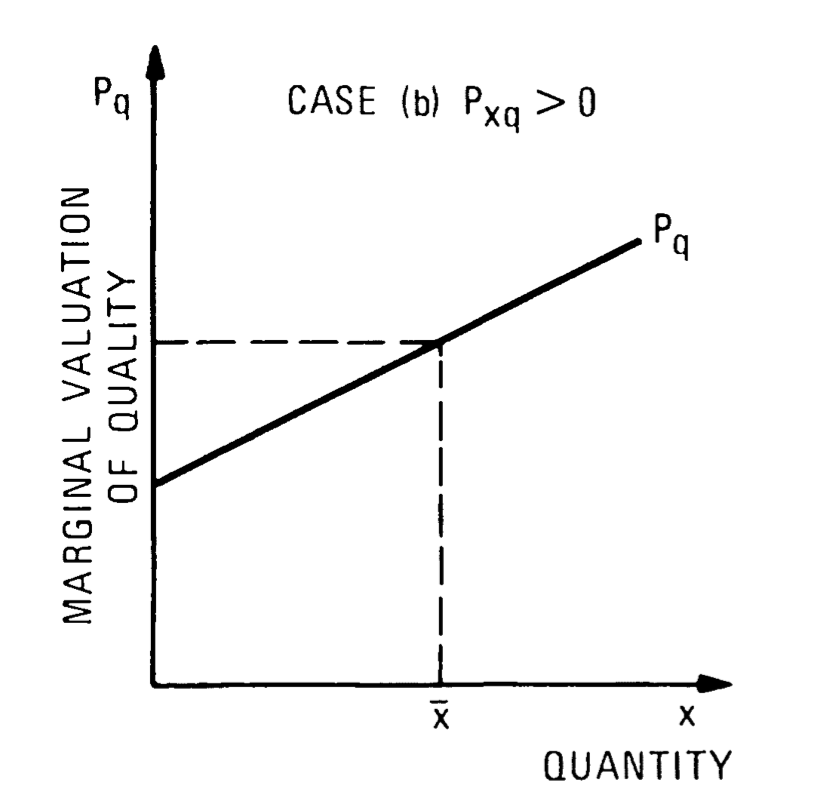
\includegraphics[width = .7\textwidth]{spence1.png}
    \label{fig:1}
\end{figure}
\end{frame}

\begin{frame}{Case 2: General Case}
Setup: 
\begin{itemize}
    \item $P_{xq}<0$, $c(x,q) = x*c(q)$ 
    \item $(\bar{x}, \bar{q})$ maximize the profit
    \item $(x^*,q^*)$ maximize the total welfare 
\end{itemize}  
\end{frame}

\begin{frame}{Case 2: General Case}
First, think of the profit maximization at $(\bar{x}, \bar{q})$:
\begin{equation}\label{eq2}
\begin{split}
\frac{\partial \pi}{\partial q} & = \bar{x} P_q(\bar{x},\bar{q}) - \bar{x}c'(\bar{q}) = 0\\
& \Rightarrow  P_q(\bar{x},\bar{q}) = c'(\bar{q})
\end{split}
\end{equation}

Then, think about the welfare maximization at $(x^*, \bar{q})$
\begin{equation}\label{eq3}
   \frac{d W}{d q}  = \int_{0}^{x^*} P_q(v,\bar{q})\,dv - x^* c'(q)
\end{equation}

Implement \ref{eq2} into \ref{eq3}, we have:
\begin{equation}
\frac{d W}{d q}  = \int_{0}^{x^*} P_q(v,\bar{q})\,dv - x^* P_q(\bar{x},\bar{q})
\end{equation}
\end{frame}

\begin{frame}{Case 2: General Case}
\begin{figure}
    \centering
    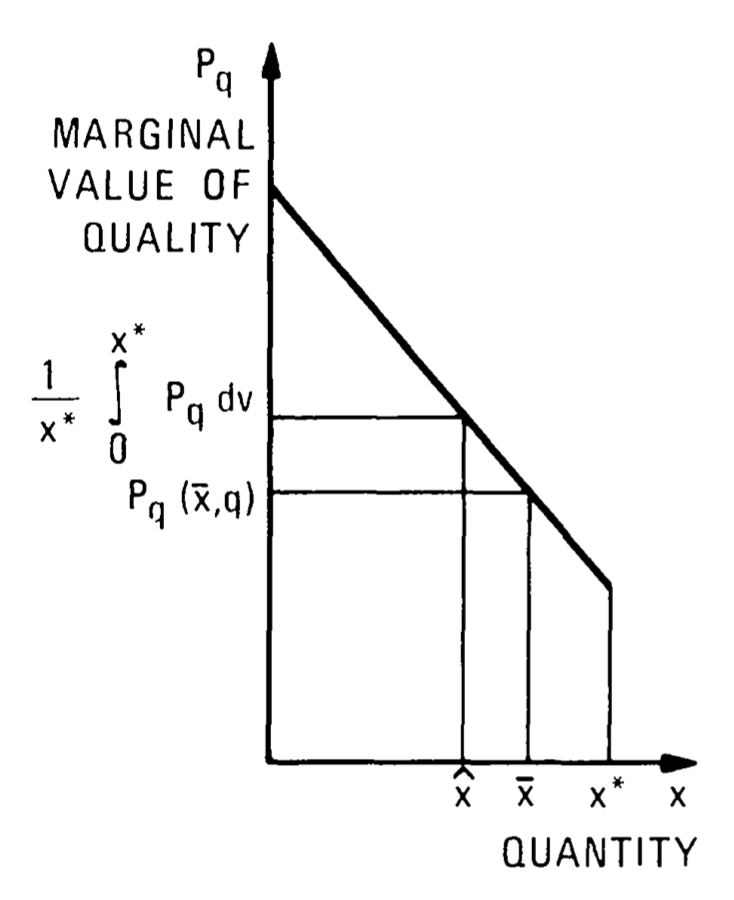
\includegraphics[width = .6\textwidth]{spence2.png}
    \label{fig:2}
\end{figure}
\end{frame}

\begin{frame}{Case 2: General Case}
Define:
\begin{equation}
    \bar{W}(q) = \max_x W(x,q) \ \ \  \bar{\pi}(q) = \max_x \pi(x,q)
\end{equation}

\begin{equation}
    \beta (q) = \frac{\bar{\pi}(q)}{\bar{W}(q)}
\end{equation}

After several steps of tedious math, we have,
\begin{equation}
    \frac{\beta'}{\beta} =\frac{\bar{\pi}'}{\bar{\pi}} - \frac{\bar{W}'}{\bar{W}}
\end{equation}

Then if $\bar{\pi}' = 0$, 
\begin{equation}
    \frac{\beta'}{\beta} = - \frac{\bar{W}'}{\bar{W}}
\end{equation}

\metroset{block=fill}\begin{block}{Proposition 2}
If $\beta'<0$, we have $\bar{W}' > 0$, which means firm undersupplies quality
\end{block}
\end{frame}

\begin{frame}{Case 2: General Case}


If we specifically set 
\begin{equation}
    P(x,q) = A(q)x^{-n(q)}
\end{equation}
and have $n'(q) >0$, i.e we have a constant price elasticity of demand and the elasticity is decreasing in quality, we can easily verify that

\begin{equation}
    \beta(q) = (1 - n(q) )^\frac{1}{n(q)} 
\end{equation}

and $\beta' < 0$.

\break

\metroset{block=fill}\begin{block}{Proposition 3}
If the price elasticity is not a function of the price and if the elasticity declines with quality, then quality is undersupplied
\end{block}
\end{frame}


\begin{frame}{First-Best Regulation}
\begin{figure}
    \centering
    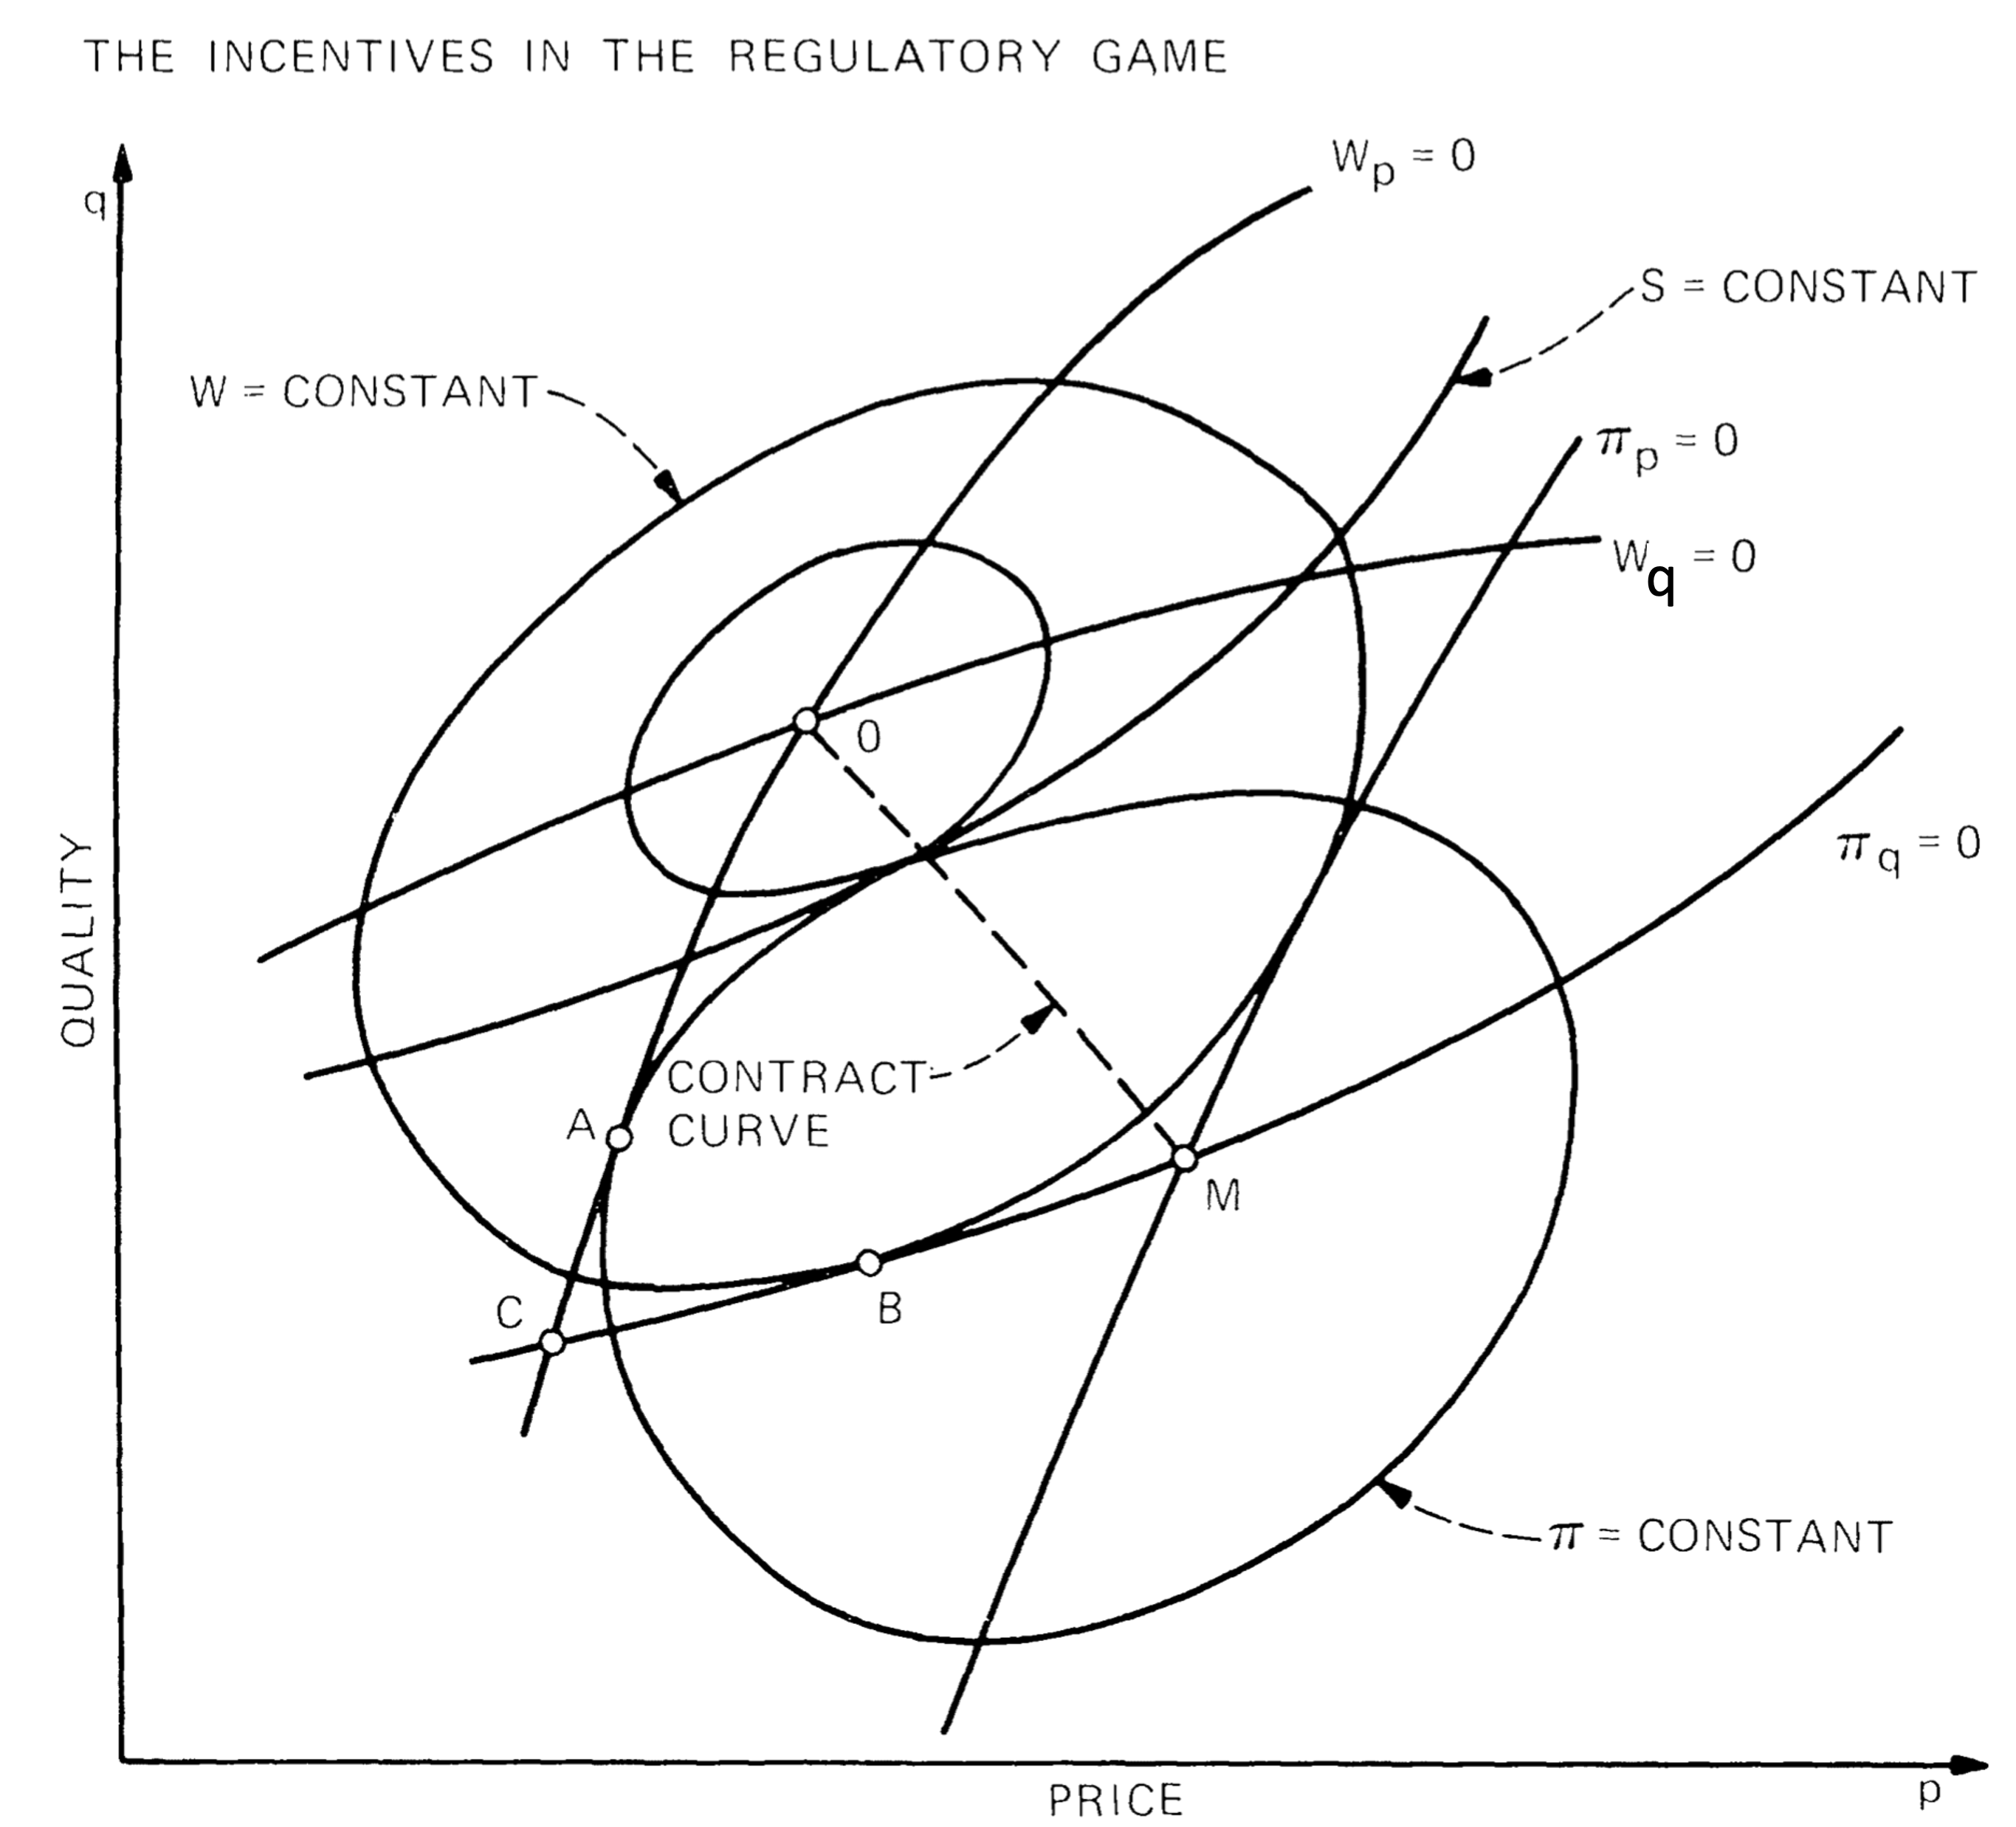
\includegraphics[width = .8\textwidth]{spence3.png}
    \label{fig:3}
\end{figure}
    
\end{frame}

\begin{frame}{First-Best Regulation}
So our first-best regulation is to set $S = s$, where s is a constant. Since $W = S + \pi$, given $S = s$, when $\pi$ is optimized, $W$ is also optimized.

$\Rightarrow$ Makes sure the solution lies on the contract curve.

However, in practice, it's hard to implement, mostly due to information limits. 

Recall
\begin{equation}
    S = \int_{p}^{\infty} D(v,q) \,dv
\end{equation}

To set the desired price-quality regulation, we need:
\begin{itemize}
    \item An accurate measure of quality
    \item The demand function D(x,q)
\end{itemize}
\end{frame}

\begin{frame}{First-Best Regulation}
To be more clear, when a regulator whether to interfere a price change, one need to access whether $dS$, the consumer surplus, is increased.
\begin{equation}
    dS = -D dp + [\int_{P}^{\infty} D_q(v,\bar{q})\,dv] dq
\end{equation}

If $dS > 0$, it is the same to have
\begin{equation}
    \frac{\int_{P}^{\infty} D_q(v,\bar{q})\,dv}{D} dq > dp
\end{equation}

On the LHS, it's the average valuation of quality change, while the RHS the price change. It's not enough to know the local demand function.
\end{frame}


\begin{frame}{Second-Best Regulation}
Now we consider putting a constrain on firm's rate of return. Let \textcolor{red}{s} be our limit rate and \textcolor{red}{$k(D,q)$} the capital employed. Simply, we have:

\begin{equation}
    \frac{pD}{k} \leq s
\end{equation}

Specifially, assume $c(x,q) = rk(D,q)$ where r is the rent of capital,
\begin{equation}
    p \leq \frac{s}{r} * \frac{c(D,q)}{D}
\end{equation}

Further, assume the average cost $\frac{c(D,q)}{D} = a(D,q)$ with $a_D \geq 0$ and $a_q > 0$, we have
\begin{equation}
    \frac{dp}{dq} = \frac{a_D D_q + a_q}{\frac{r}{s} - a_D D_p} > 0
\end{equation}
\end{frame}

\begin{frame}{Second-Best Regulation}
So like the first-best regulation, the rate of return regulation also set an up sloping curve in price-quality space, and its slope is determined by s and r.

But in this case, we can't be sure the solution lies on the contract curve, thus we will have some efficiency loss.
\end{frame}

\begin{frame}{Second-Best Regulation}
\begin{figure}
    \centering
    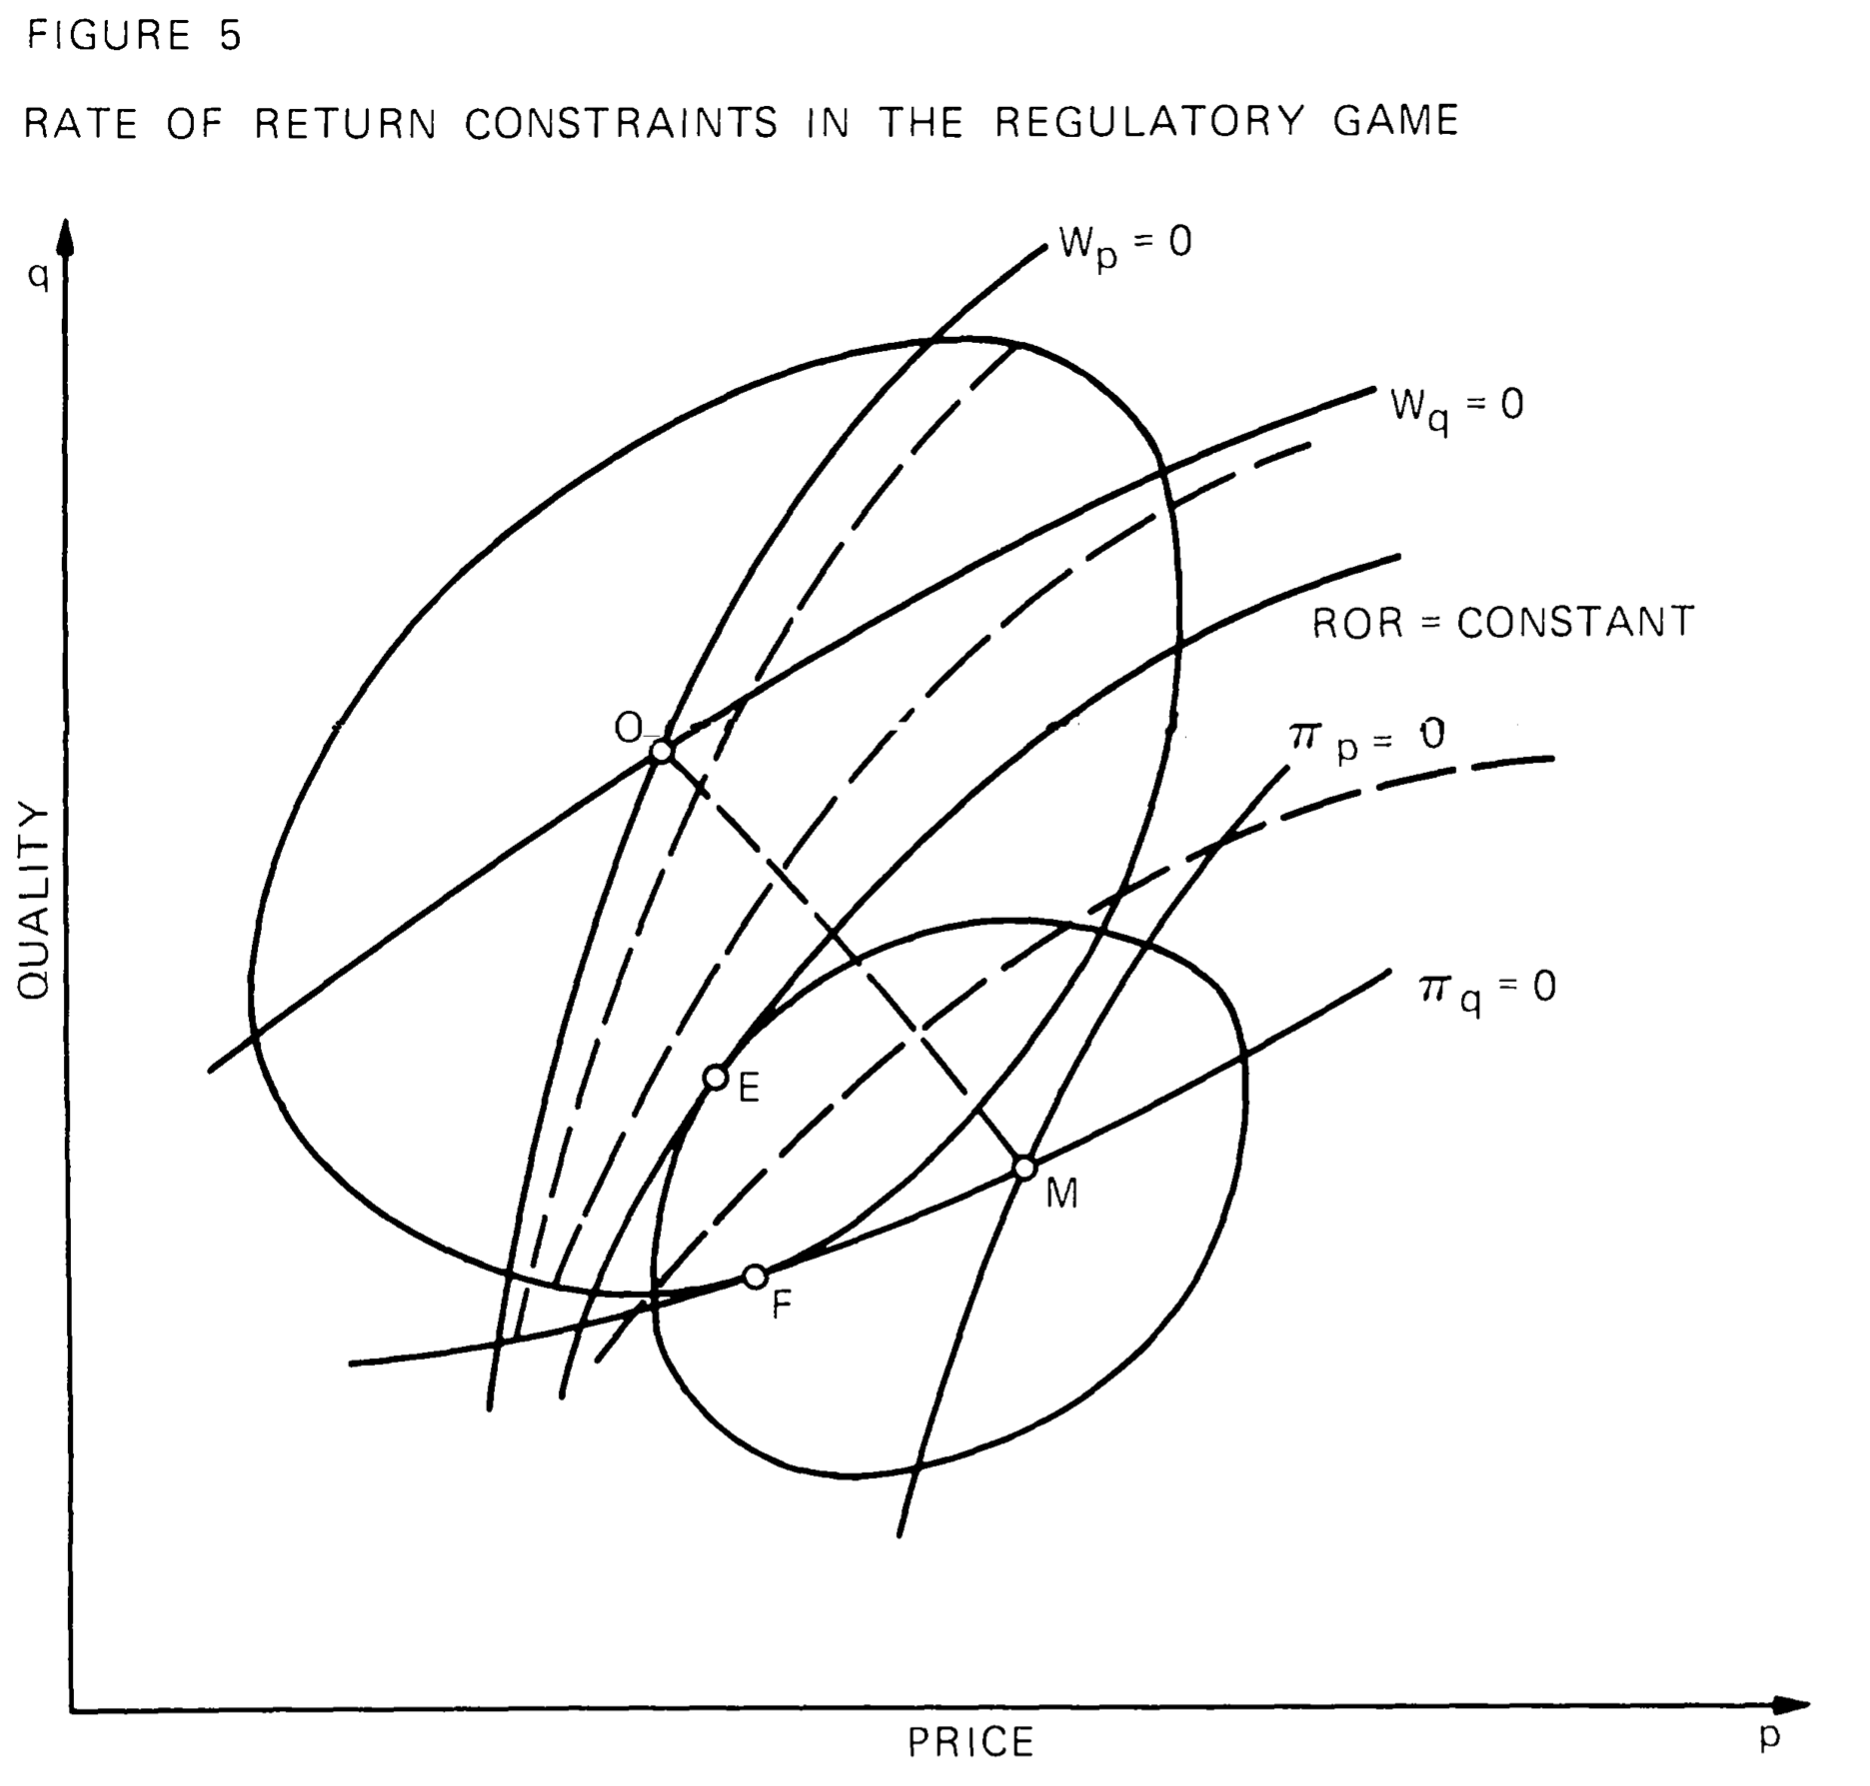
\includegraphics[width = .8\textwidth]{spence4.png}
    \label{fig:my_label}
\end{figure}
\end{frame}

\begin{frame}{Summary}
    So what do we learn from this one:
\begin{enumerate}
    \item In a monopoly market, \textcolor{red}{quality is usually less supplied}
    \item Ideally, the regulator can set a price-quality standard according to a constant consumer surplus. But that requires knowledge of valuation distribution across all the market.
    \item Rate of return regulation has some merit in these circumstances as a second-best strategy, especially when (1) profit maximizing quality tends to be too low and (2) quality is a capital-using attribute.
\end{enumerate}
\end{frame}


\subsection{Market Equilibrium with Quality Difference}
\begin{frame}{Introduction to Shaked \& Sutton(1982)}
In this part we will focus on Shaked \& Sutton(1982).
This paper employed a 3-staged game to find a market equilibrium when there are quality differences among products.
\begin{figure}
    \centering
    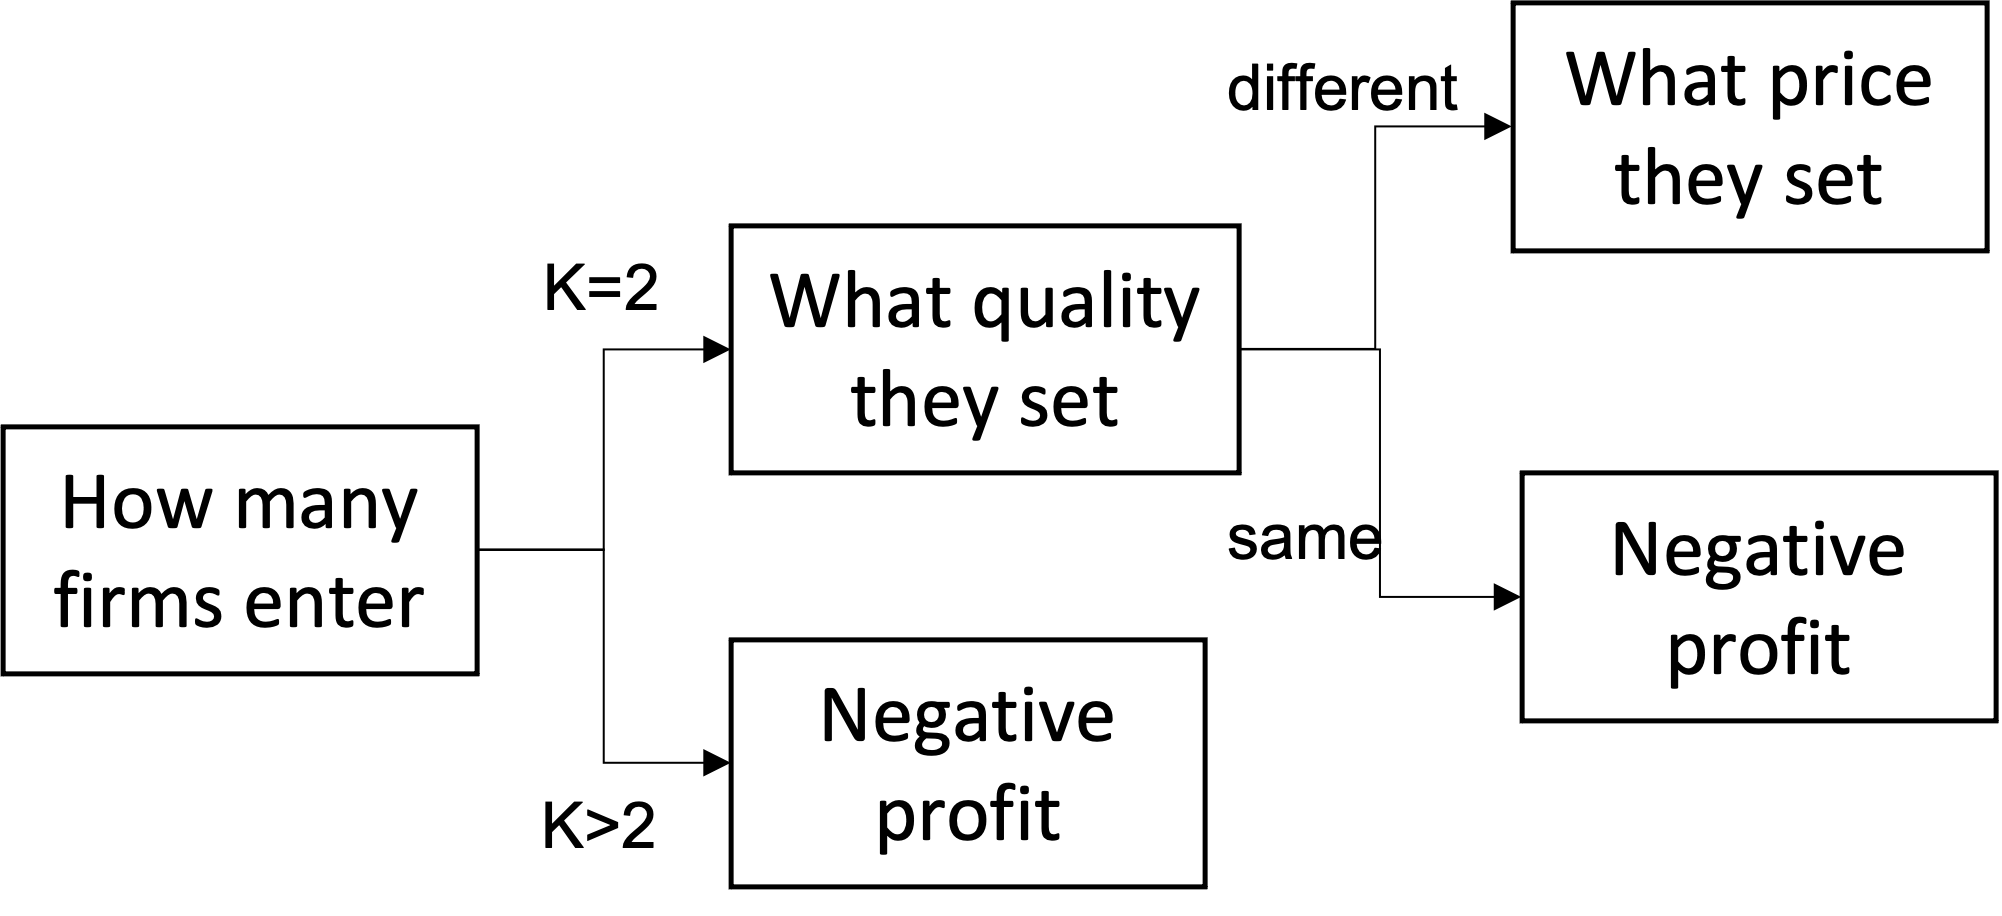
\includegraphics[width = .7\textwidth]{shaked1.png}
\end{figure}
To solve this game, we need to use backward induction, so let's look at the last part--price competition
\end{frame}

\begin{frame}{Tour Guide}
\begin{figure}
    \centering
    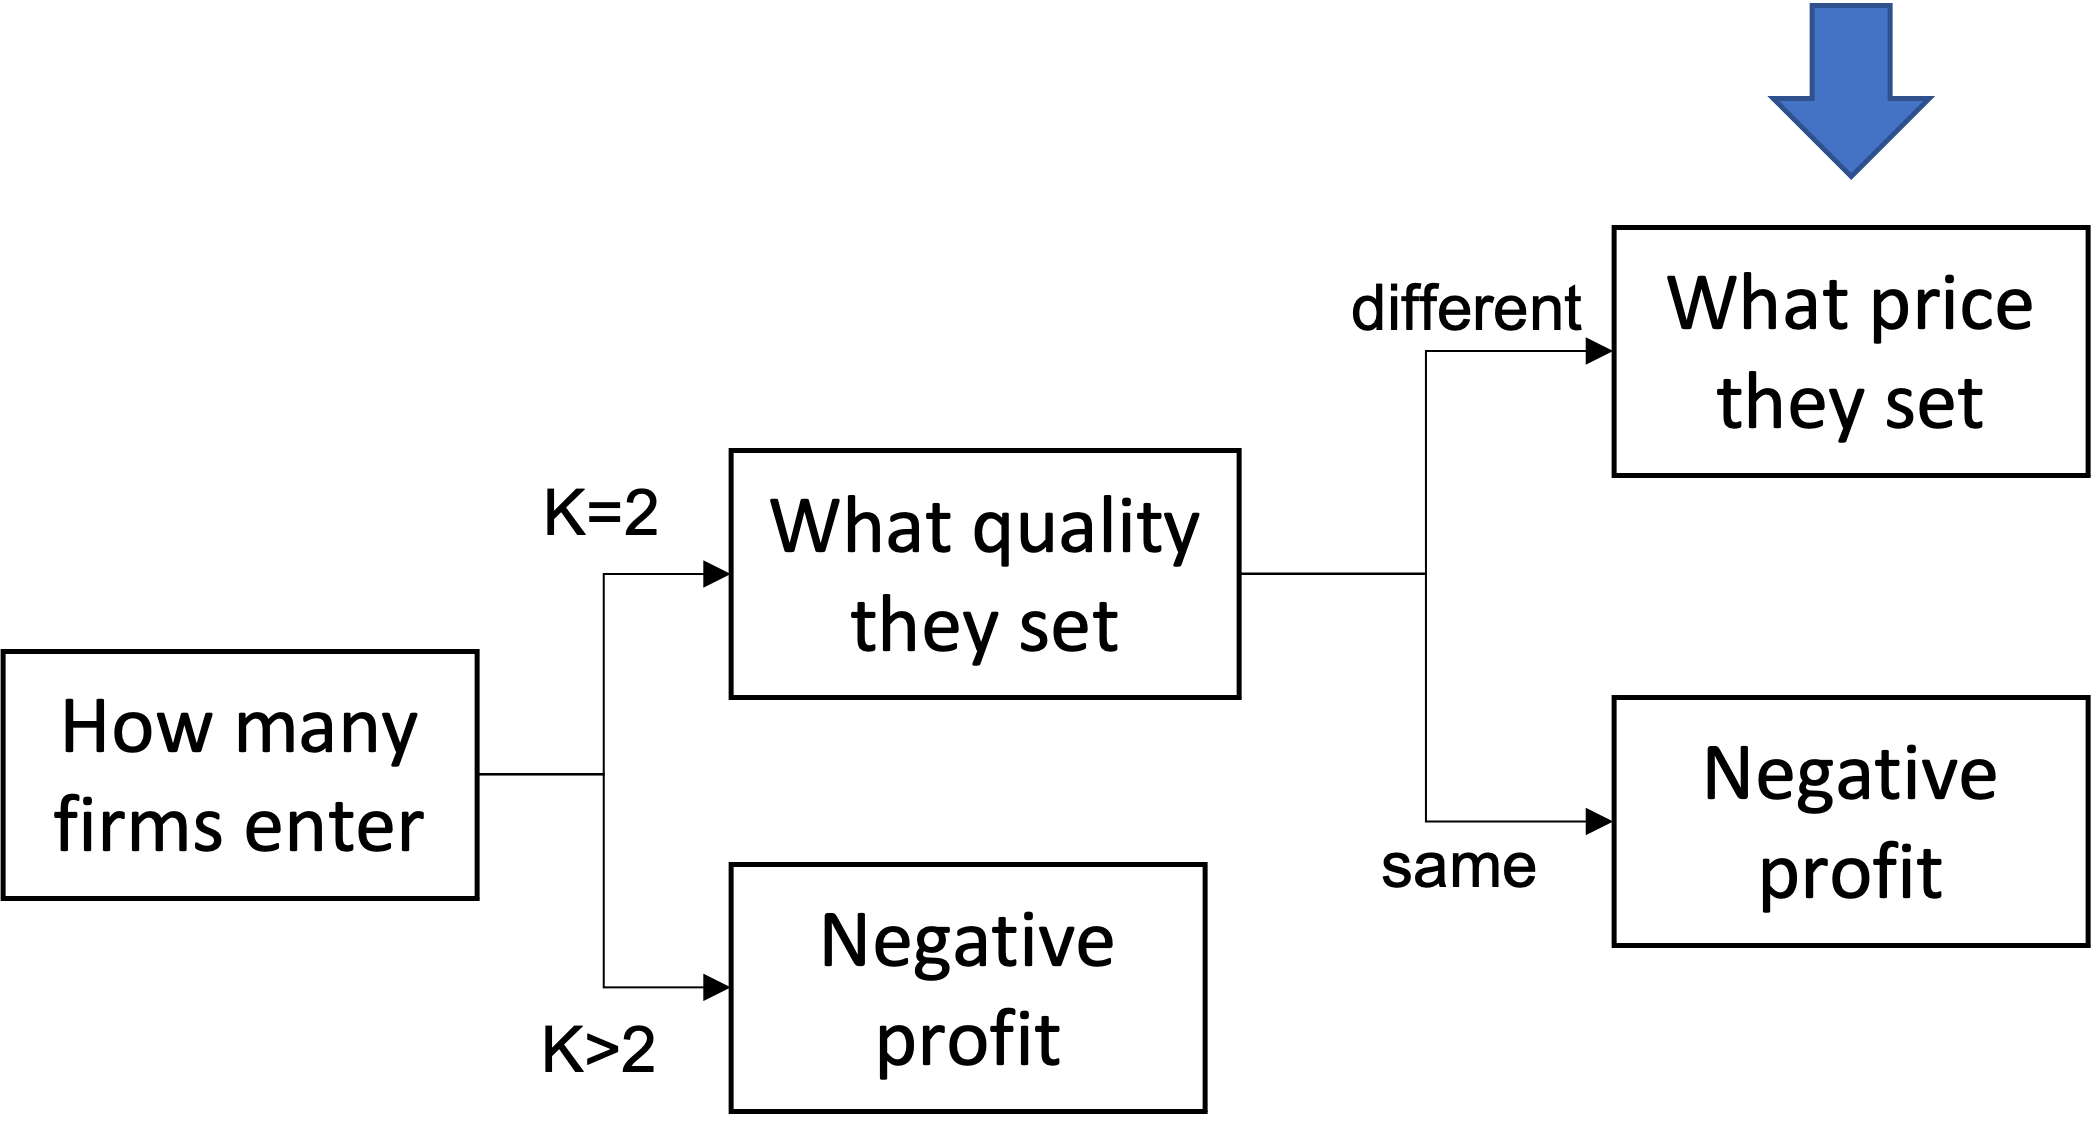
\includegraphics[width = .9\textwidth]{guide1.png}

\end{figure}
    
\end{frame}
\begin{frame}{Price Competition}
Setup:
\begin{itemize}
    \item We have $n$ number of distinct, substitute products, indexed by $k = 1,...,n$ at prices $p_k$
    \item Have a order of quality as $u_0 < u_1 <... < u_n$ where $u_0$ is the utility for outside option
    \item There exist a continuum of consumer with same preference but different income. Let they have income uniformly distributed. $t \in [a,b]$ s.t. $a > 0$
    \item Consumer can only buy 1 or none product
\end{itemize}
Define their utility function as:
\begin{equation}
    U(t,k) = u_k \cdot t
\end{equation}

    
\end{frame}

\begin{frame}{Price Competition}
Define several income level $t_k$, and assume that consumer with income $t_k$ is indifferent from product $k$ and $k-1$.
\begin{equation}
    U(t_k - p_k,k) = U(t_{k-1} - p_{k-1}, k-1)
\end{equation}

Than we can solve $t_k$ as a function of $u_k, u_{k-1}, p_k, p_{k-1}$
\begin{equation}
    \begin{split}
        & t_1 = p_1 C_1 \\
        & t_k = p_{k-1}(1 - C_k) + p_k C_k
    \end{split}
\end{equation}
where
\begin{equation}
    C_k = \frac{u_k}{u_k - u_{k-1}}
\end{equation}
Obviously, $C_k > 1 $, and consumer with $t > t_k$ would strictly prefer product $k$ to product $k-1$.
\end{frame}

\begin{frame}[t]{Price Competition}
To better understand $t_k$, which is the key to this analysis, let's have some examples. Consider a case with 2 distinct products.
\break

\begin{tikzpicture}[remember picture, overlay]
\node[] at (current page.center) 
{
    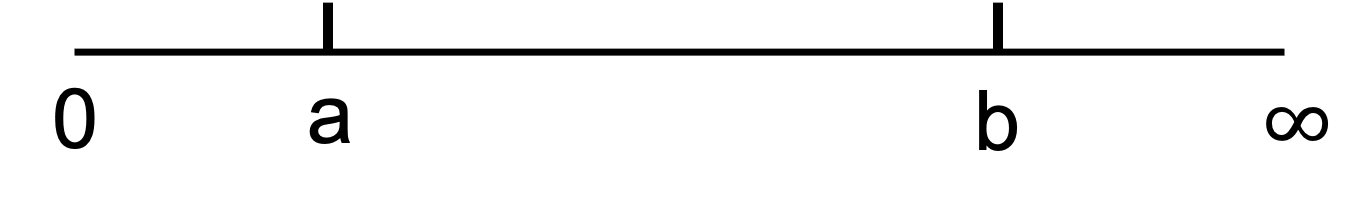
\includegraphics[width = .7\textwidth]{sk2.png}
};
\end{tikzpicture}

\begin{tikzpicture}[remember picture, overlay]
\node[above = 1.2cm] at (current page.south) 
{
    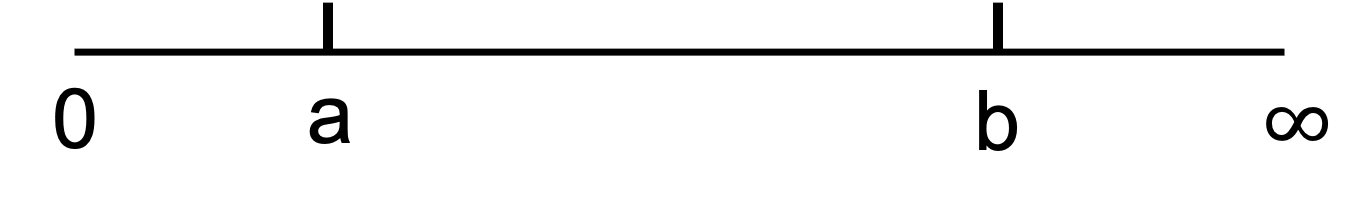
\includegraphics[width = .7\textwidth]{sk2.png}
};
\end{tikzpicture}
\end{frame}

\begin{frame}{Price Competition}
Now let's look at the firms. 

Assume no cost, the profits equal revenue. 

Since consumes' income is uniformly distributed, $(t_k - t_{k-1})$ is a segment of the market.
\begin{equation}
\begin{split}
& R_1 = \left\{ 
\begin{array}{@{}l@{\thinspace}l}
p_1(t_2 - a) &:  t_1 \leq a\\
p_1(t_2 - t_1) &:  t_1 > a\\
\end{array}
\right.\\
& R_k = p_k(t_{k-1} - t_k) \ \ , \ \ k = 2,..., n-1\\
& R_n = p(b - t_n) \\
\end{split}
\end{equation}
\end{frame}

\begin{frame}{Price Competition}
Then let's find the FOCs for each firm. Note they can only set their own price.

for $k = 1$
\begin{equation}
    \begin{split}
        t_2 - a - p_1(C_2 - 1 ) = 0  & : t_1 < a \\
        t_2 - t_1 -p_1(C_2 + C_1 -1) = 0 &: t_1 \geq a
    \end{split}
\end{equation}


for $k = 2,..., n-1$
\begin{equation}
    t_{k+1}-t_k - p_k(C_{k+1} + C_k - 1) = 0
\end{equation}

for $k = n$
\begin{equation}
    b - t_n - p_n C_n = 0
\end{equation}
\end{frame}

\begin{frame}{Price Competition}
Now let's make the math even messier by rewriting the FOCs for $k \geq 2$.
\begin{equation}
\begin{split}
        t_{k+1} -2t_k &= p_k(C_{k+1} - 1) + p_{k-1}(C_k -1)   \\
             b -2t_n &= p_{n-1} (C_n -1)  \\
\end{split}
\end{equation}

Recall that $C_k >1 \ \forall \ k$, we have

\begin{equation}
    b > 2 t_n \ , \  t_{k+1} >2 t_k
\end{equation}
\begin{equation}
    \Rightarrow 4t_{n-1} < b
\end{equation}
\metroset{block=fill}
\begin{block}{Lemma 1}
Let $b < 4a$. Then for any Nash Equilibrium involving the distinct goods
$n$, $n - 1$, ..., $1$ at most two products (the top two) have a positive market share at equilibrium. 
\end{block}
\end{frame}

\begin{frame}[t]{Price Competition}
With $b < 4a$, we have $t_{n-1} < a$, which means there exist only 3 kinds of consumer, one prefers $n-1$, one prefers $n$, and one indifferent.

\break
\begin{tikzpicture}[remember picture, overlay]
\node[above = 2cm] at (current page.south) 
{
    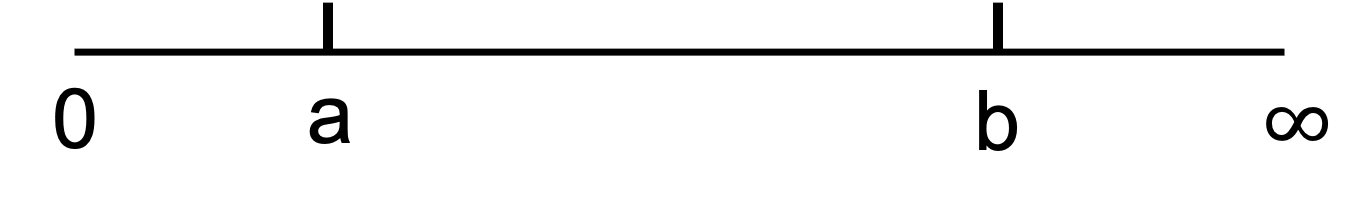
\includegraphics[width = .8\textwidth]{sk2.png}
};
\end{tikzpicture}
\end{frame}

\begin{frame}{Price Competition}
Then, based on lemma 1, let's solve for the equilibrium when $n = 2$. Traditionally, a pair of price $(p_1, p_2)$ can define a equilibrium, but here we are looking for income level $(t_1,t_2)$. They're essentially the same.

For simplicity, define
\begin{equation}
    V = \frac{u_2 - u_0}{u_2 - u_1} = \frac{C_2 - 1}{C_1} + 1
\end{equation}

Obviously, $V > 1$. Then we can rewrite the FOCs as

Firm 1:
\begin{equation}
    \begin{split}
        t_2 = a + t_1 (V - 1) &: t_1 \leq a\\
        t_2 = t_1(V + 1) &: t_1 \geq a \\
    \end{split}
\end{equation}

Firm 2:
\begin{equation}
    b- 2t_2 = t_1(V - 1)
\end{equation}
\end{frame}

\begin{frame}{Price Competition}
In the $t_2-t_1$ space, the FOC of firm 1 gives us a up sloping piecewise line while it of firm 2 gives a down sloping line

\begin{figure}
    \centering
    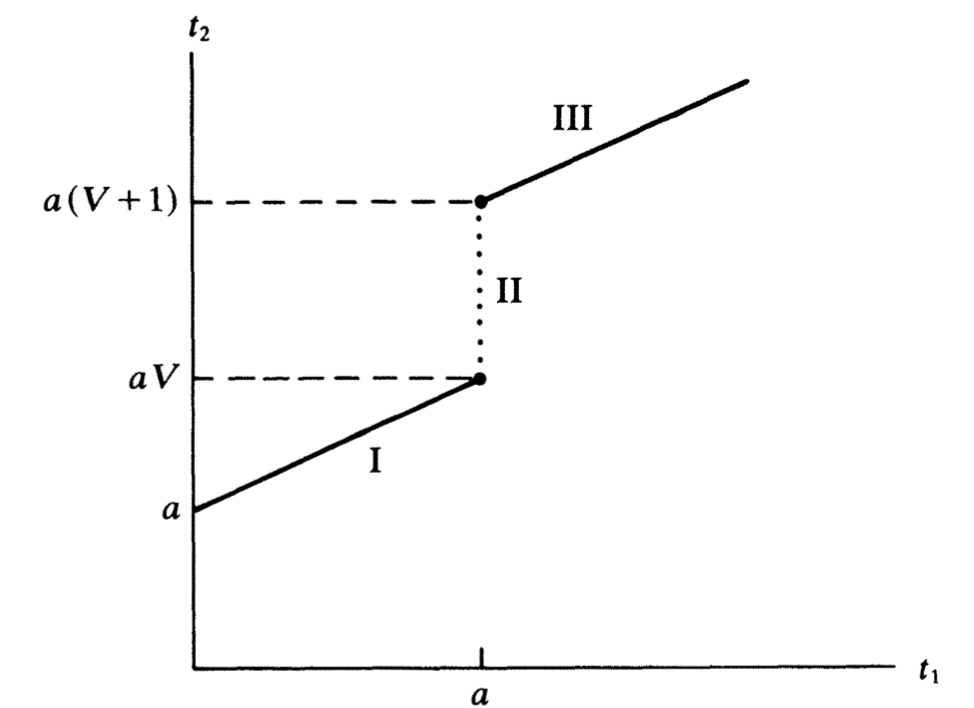
\includegraphics[width = .7\textwidth]{sk3.png}
\end{figure}
    
\end{frame}

\begin{frame}{Price Competition}
After solving for $(t_1,t_2)$, we can find that the location of the point is determined by V, and eventually by $u_2 - u_1$. 
\begin{equation}
    \begin{split}
        \text{Region I}   &: V \geq \frac{b+a}{3a} \\
        \text{Region II}  &: V \in [\frac{b-a}{3a}, \frac{b+a}{3a}] \\
        \text{Region III} &: V \leq \frac{b-a}{3a} \\
    \end{split}
\end{equation}
If the solution lies in region III, then $t_1 > a$, which means all the consumers with $t$ $\in$ $[a, t_1]$ will choose to buy nothing(outside option), so the market is not covered.
\pause
\metroset{block = fill}\begin{block}{Lemma 2}
Let $2a < b < 4a$. Then of any $n$ firms offering distinct products, exactly two will have positive market shares at equilibrium. Moreover, at equilibrium, the market is covered.
\end{block}
\end{frame}

\begin{frame}{Tour Guide}
\begin{figure}
    \centering
    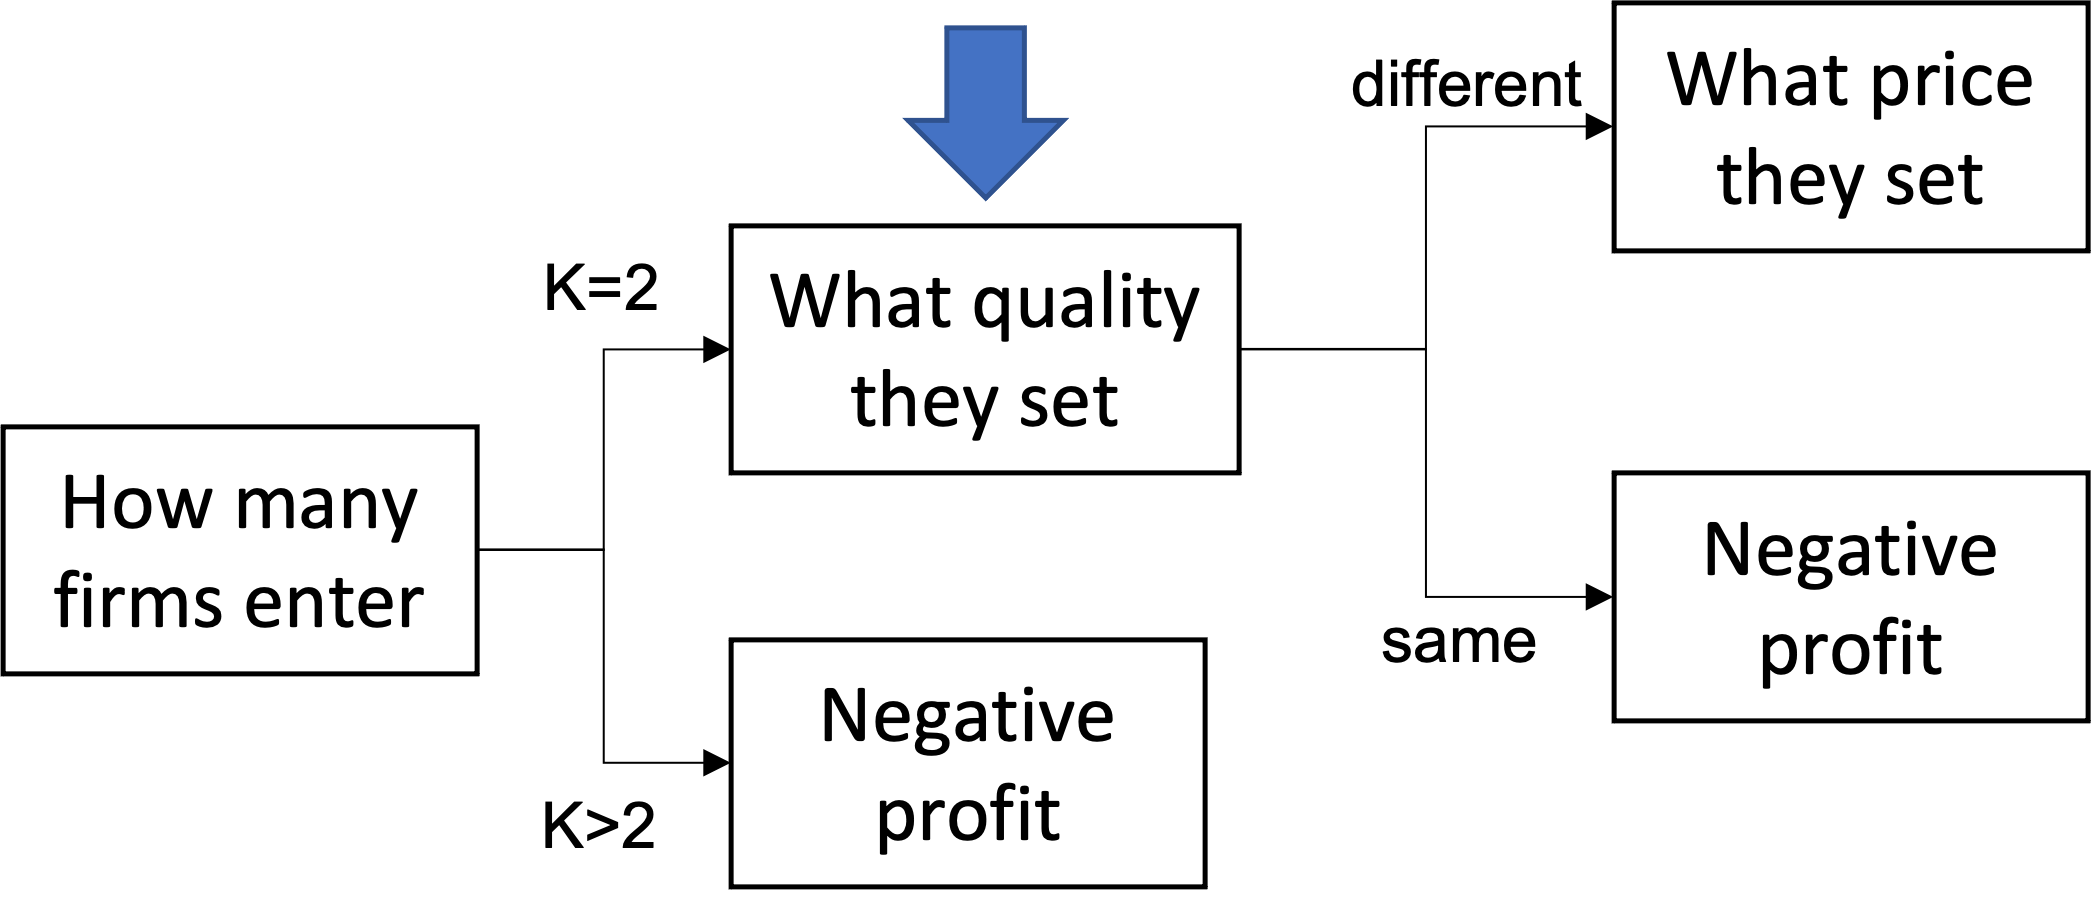
\includegraphics[width = .9\textwidth]{guide2.png}

\end{figure}
\end{frame}

\begin{frame}{Quality Competition}
From now on, we allow firms to select their quality $u_i$ $\in$ $[u_0, \bar{u}]$. But we restricted the number of firms to be 2.

Denote their equilibrium revenue $R(u,v)$ as a function of their quality $u$ and the rival's quality $v$.

\metroset{block = fill}\begin{block}{Lemma 3}
For any two qualities $u > v$, the top quality firm enjoys greater revenue than its rival, i.e.
\begin{equation}
    R(u,v) > R(v, u)
\end{equation}
\end{block}

\metroset{block=fill}\begin{block}{Lemma 4}
The revenues of both firms increase as the quality of the better product improves, i.e., $ R_u(v,u) > 0$ and $R_u(u,v) > 0$
\end{block}
\end{frame}

\begin{frame}{Quality Competition}
Now let's think about the quality-setting strategies of firms. Let one firm set their quality first, and his rival will set a lower quality that maximize their revenue. 

Moreover, let's assume that $R(v,u) = 0$ if $v = u$, and $R(v,u) > 0 $ if $v < u$.

Define ``the optimal reply from the below":
\begin{equation}
    \rho(u)= \{ v \in [u_0,u] \ | \ v = arg\max_s R(s,u) \}
\end{equation}

\end{frame}

\begin{frame}{Quality Competition}
Claim: $(\rho(\bar{u}), \bar{u})$ is a Nash equilibrium. Index the firm with lower quality firm 1, and the other firm 2

For firm 1, any $u_1 \neq  \rho(\bar{u})$ generate less revenue
\begin{equation}
    R(\rho(\bar{u}), \bar{u}) > R(u_1, \bar{u})
\end{equation}
For firm 2, any $u_2 \neq \bar{u}$ generate less revenue
\begin{equation}
    R(\bar{u}, \rho(\bar{u})) > R(u_2, \rho(\bar{u}))
\end{equation}

\metroset{block = fill}\begin{block}{Proposition I}
The game has a perfect equilibrium in pure strategies; the outcome involves distinct qualities, and both firms earn positive revenue (profits) at equilibrium
\end{block}
\end{frame}


\begin{frame}{Quality Competition}
Now, let's look at cases where the number of firms is $k > 2$.

Claim: A Nash equilibrium is $u_i = \bar{u}$ for all $i = 1,..., k$.

It suffices to show that the benefit of deviation is not greater than it of commitment.

If all the firms but one adopt $\bar{u}$, as a result of Bertrand competition, they would set price = MC = 0, so the benefit of deviation can not be larger than 0

\metroset{block = fill}\begin{block}{Proposition II}
(i) When $k > 2$, the game has a Nash Equilibrium $u_i = \bar{u}$, $\forall$ $i = 1,...,k$.
(ii) For every Nash Equilibrium, the payoff for each firm is zero.
\end{block}
\end{frame}

\begin{frame}{Tour Guide}
\begin{figure}
    \centering
    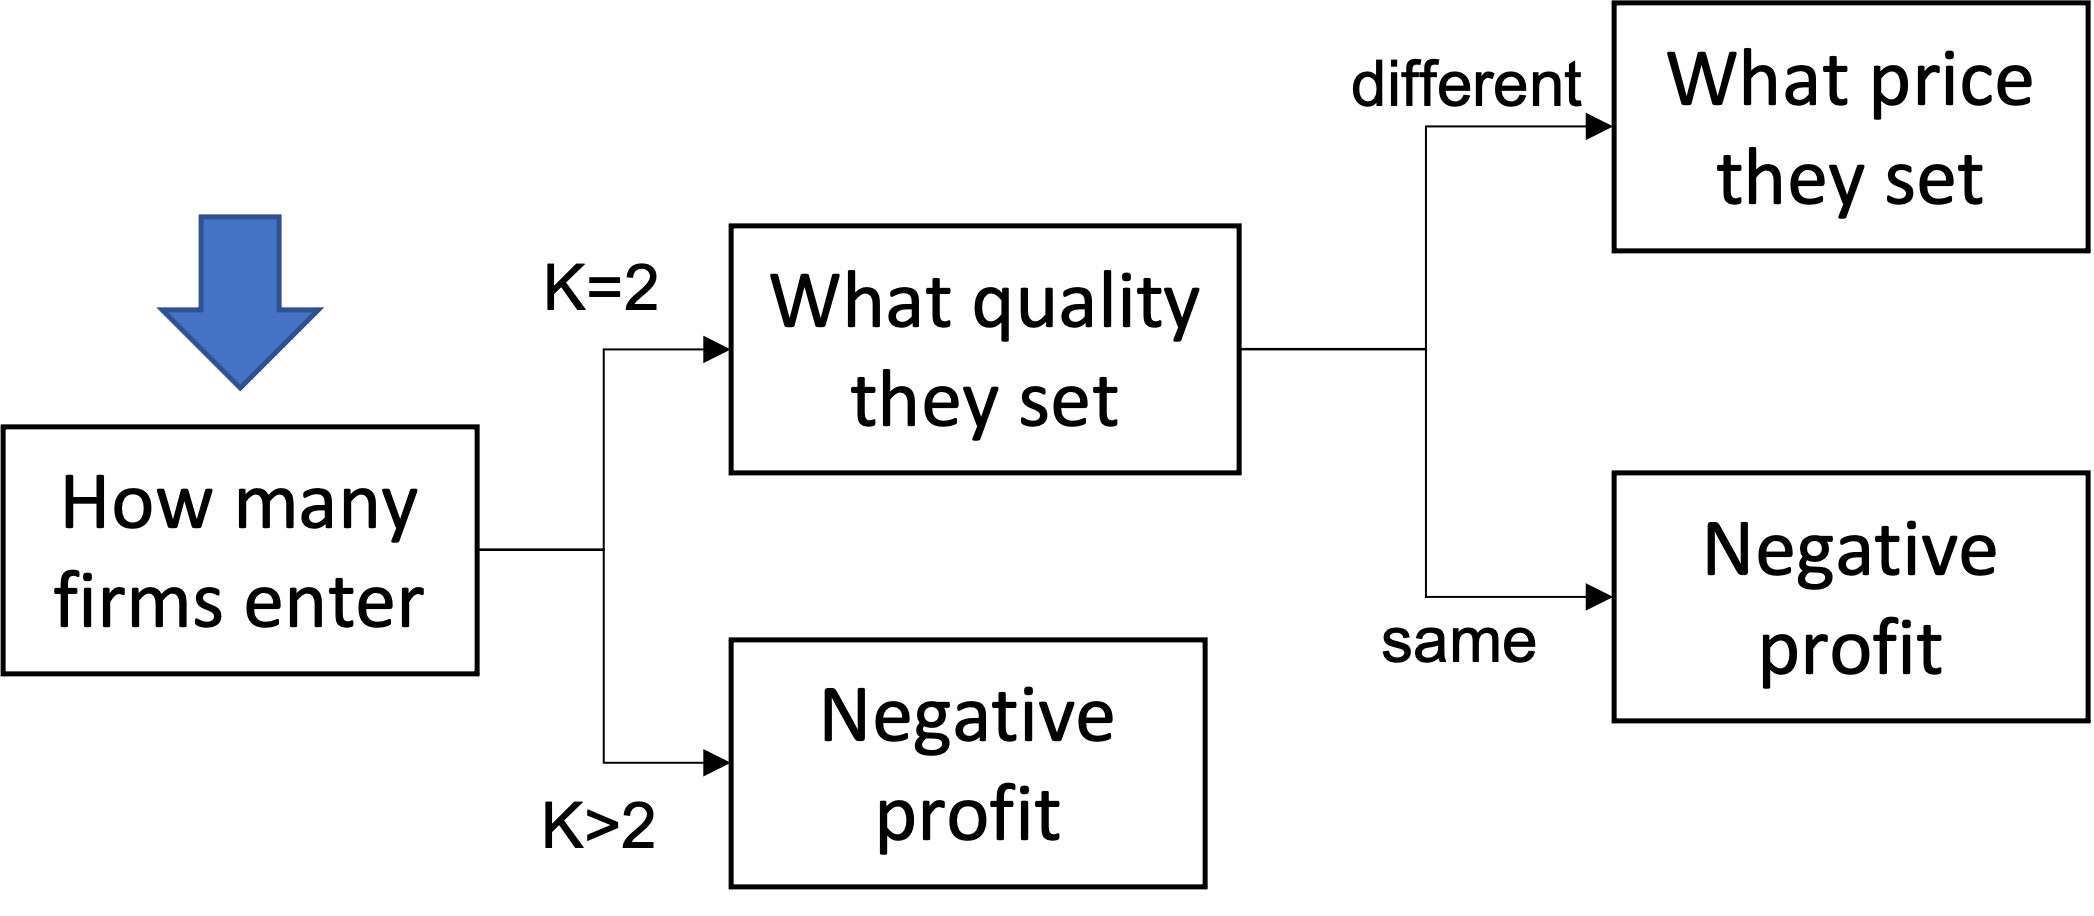
\includegraphics[width = .9\textwidth]{guide3.png}

\end{figure}
\end{frame}

\begin{frame}{Entry}
\metroset{block = fill}\begin{block}{Proposition III}
For any $\epsilon >0 $ (sufficiently small), and any number $n > 2$ of potential entrants:\\
\begin{enumerate}
    \item There exists a Perfect Equilibrium in which two firms enter; and in which they produce distinct products, and have positive revenues (profits).
    \item No Perfect Equilibrium exists in which $k > 2$ firms enter
\end{enumerate}
\end{block}
\end{frame}

\begin{frame}{Summary}
\begin{figure}
    \centering
    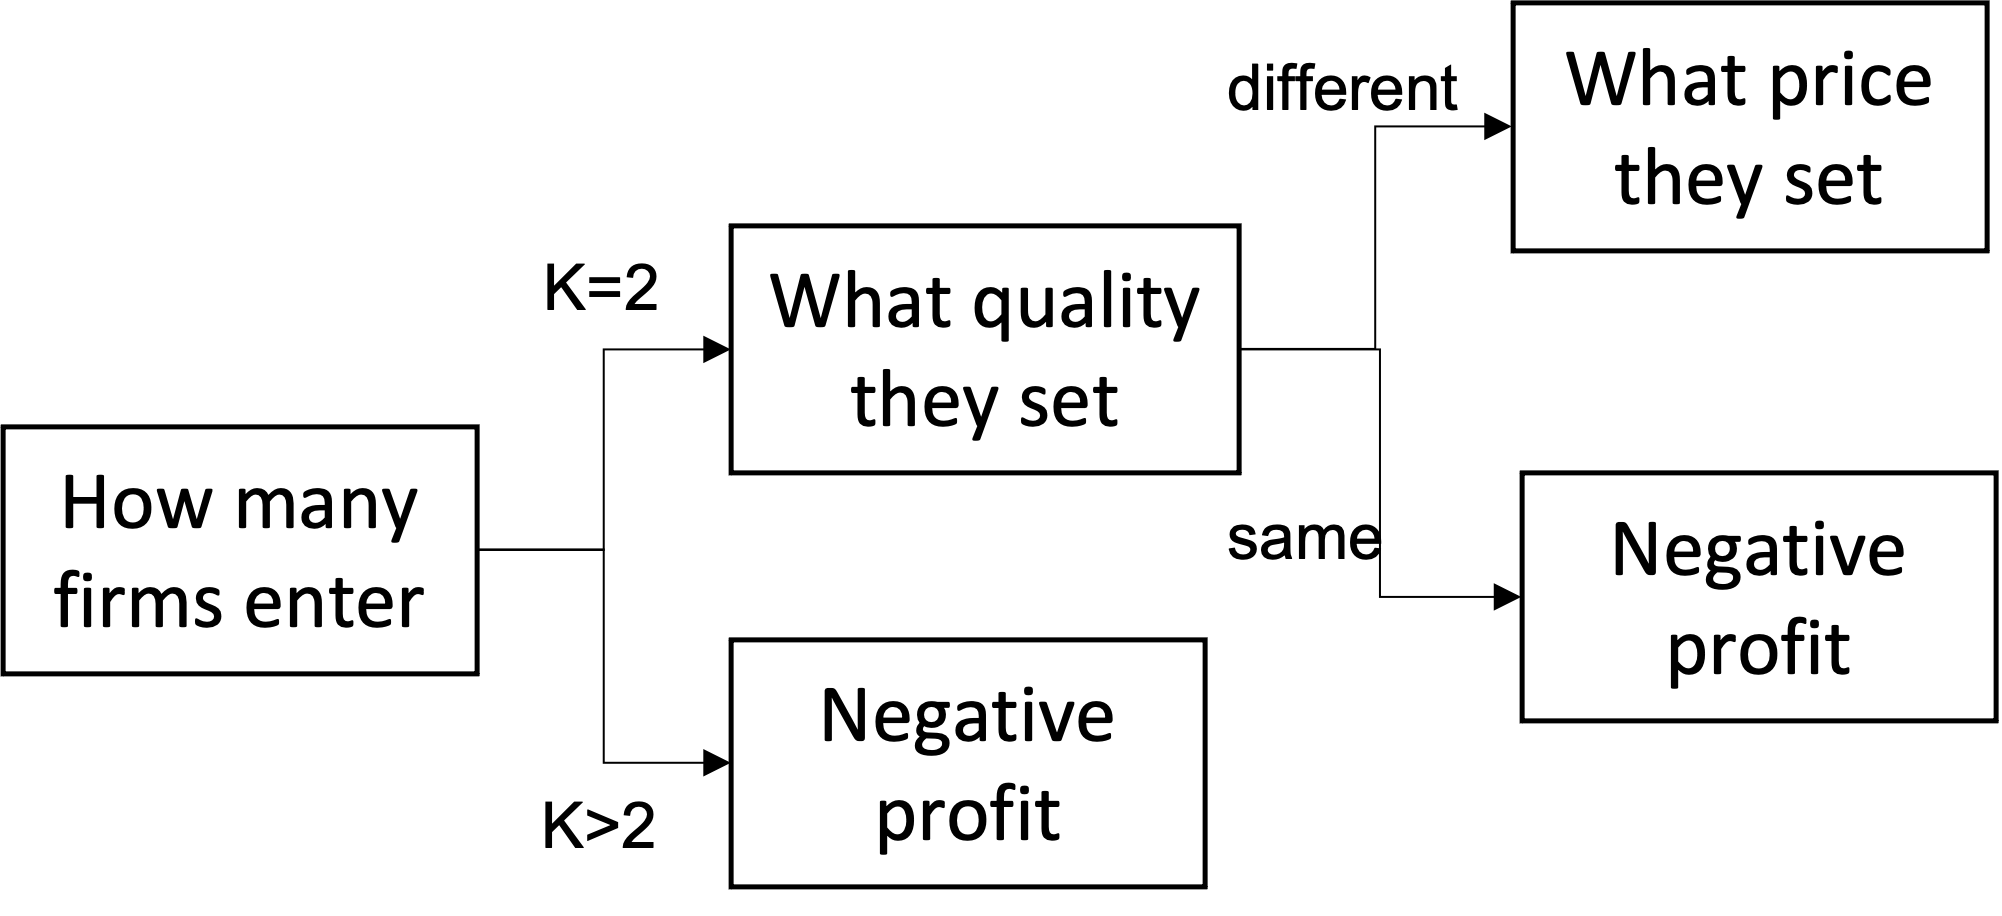
\includegraphics[width = .8\textwidth]{shaked1.png}
    \label{fig:sk1}
\end{figure}
    
\end{frame}






\section{Advertising}

\subsection{Views on Advertising}
\begin{frame}{Views on Advertising}
Before doing any analysis of advertising, the primary question is: why(how) people response to advertisement?

There are 3 main views on advertising: persuasive, informative, and complementary.
\end{frame}

\begin{frame}{Persuasive View}
The persuasive view, in general, sees advertising as a problem
\begin{itemize}
    \item Advertising can \textcolor{red}{distort consumer's preference}, so as to move the demand curve upwards or make it inelastic.
    \item It can build brand loyalty, and therefore \textcolor{red}{raise the entry barrier}
    \item It has \textcolor{red}{no real value} to consumers
\end{itemize}

All together, advertising will make the market more concentrated with higher price and profit.
\end{frame}
 
 
\begin{frame}{Informative View}
Though many aspects of persuasive view is reasonably matched with reality, it doesn't explain why firms in highly competitive market would advertise.

In the informative view, advertising is valuable to consumers as it can reduce search cost. This view relies heavily on information economics.
\begin{itemize}
    \item Advertisement \textcolor{red}{contains valuable information} which can reduce consumer's search cost.
    \item Even for some advertisement which doesn't contain information about the product, they can \textcolor{red}{provide valuable indirect information}.
\end{itemize}
\end{frame}

\begin{frame}{Complementary View}
Informative view explains to a large extent why competitive firms advertise, but we can see a lot of advertisement contains no information about the product at all.

Under this view, advertisement is a complementary of the consumed product and can generate utility.

\begin{itemize}
    \item Consumption utility is generated by the \textcolor{red}{composite commodity} of the market good and advertising.
    \item Given the \textcolor{red}{complementarity} between advertising and the market good in the production of utility, the good is more attractive when there is more advertisement.
\end{itemize}
\end{frame}


\subsection{Positive Analysis of Advertising}
\begin{frame}{Introduction}
Dorfman and Steiner(1954) provide us with an useful model of describing advertising for a monopoly firm.

Setup: 
\begin{itemize}
    \item Firms decide on the price $p$ and intensity of advertising $A$
    \item The demand function is $Q(p,A)$, with $Q_p <0$ and $Q_A > 0$
    \item Profit 
    \begin{equation}
        \pi(p,A) = p Q(p,A) - C(Q(p,A)) - A
    \end{equation}
\end{itemize}
\end{frame}

\begin{frame}{Dorfman-Steiner}
Then, let's find the FOCs for price and advertising:
\begin{equation}
\begin{split}
\frac{\partial \pi}{\partial p} = Q + (p - C')Q_p &= 0 \\
\Rightarrow \frac{p-C'}{p} = - \frac{Q}{p Q_p} &= \frac{1}{\epsilon_{Q,p}} \\
\end{split}
\end{equation}
\begin{equation}
\begin{split}
\frac{\partial \pi}{\partial A} = (p-C')Q_A - 1 &= 0 \\
\Rightarrow \frac{p-C'}{p} = \frac{1}{p Q_A} &= \frac{Q}{A Q_A} \cdot \frac{A}{pQ}\\
&= \frac{1}{\epsilon_{Q,A}} \cdot \frac{A}{p Q}
\end{split}
\end{equation}
\end{frame}

\begin{frame}{Dorfman-Steiner}
Now equating the markups, we have
\begin{equation}
\begin{split}
\frac{1}{\epsilon_{Q,p}} &= \frac{1}{\epsilon_{Q,A}} \cdot \frac{A}{p Q} \\
\Rightarrow \frac{\epsilon_{Q,A}}{\epsilon_{Q,p}} &= \frac{A}{p Q} \\
\end{split}
\end{equation}
\end{frame}

\subsection{Normative Analysis of Advertising}
\begin{frame}{Introduction to Dixit \& Norman(1978)}
In this part we go a little bit further to the welfare effect of advertising.

Their view of advertising is in accordance with the persuasive view that the consumer's preference can be distorted by advertising.

A key issue here is the welfare standard when doing the comparison. We need to identify \textcolor{red}{consumers who would not buy without the advertising}. 
\end{frame}

\begin{frame}{Graphic Intuition}
\begin{figure}
    \centering
    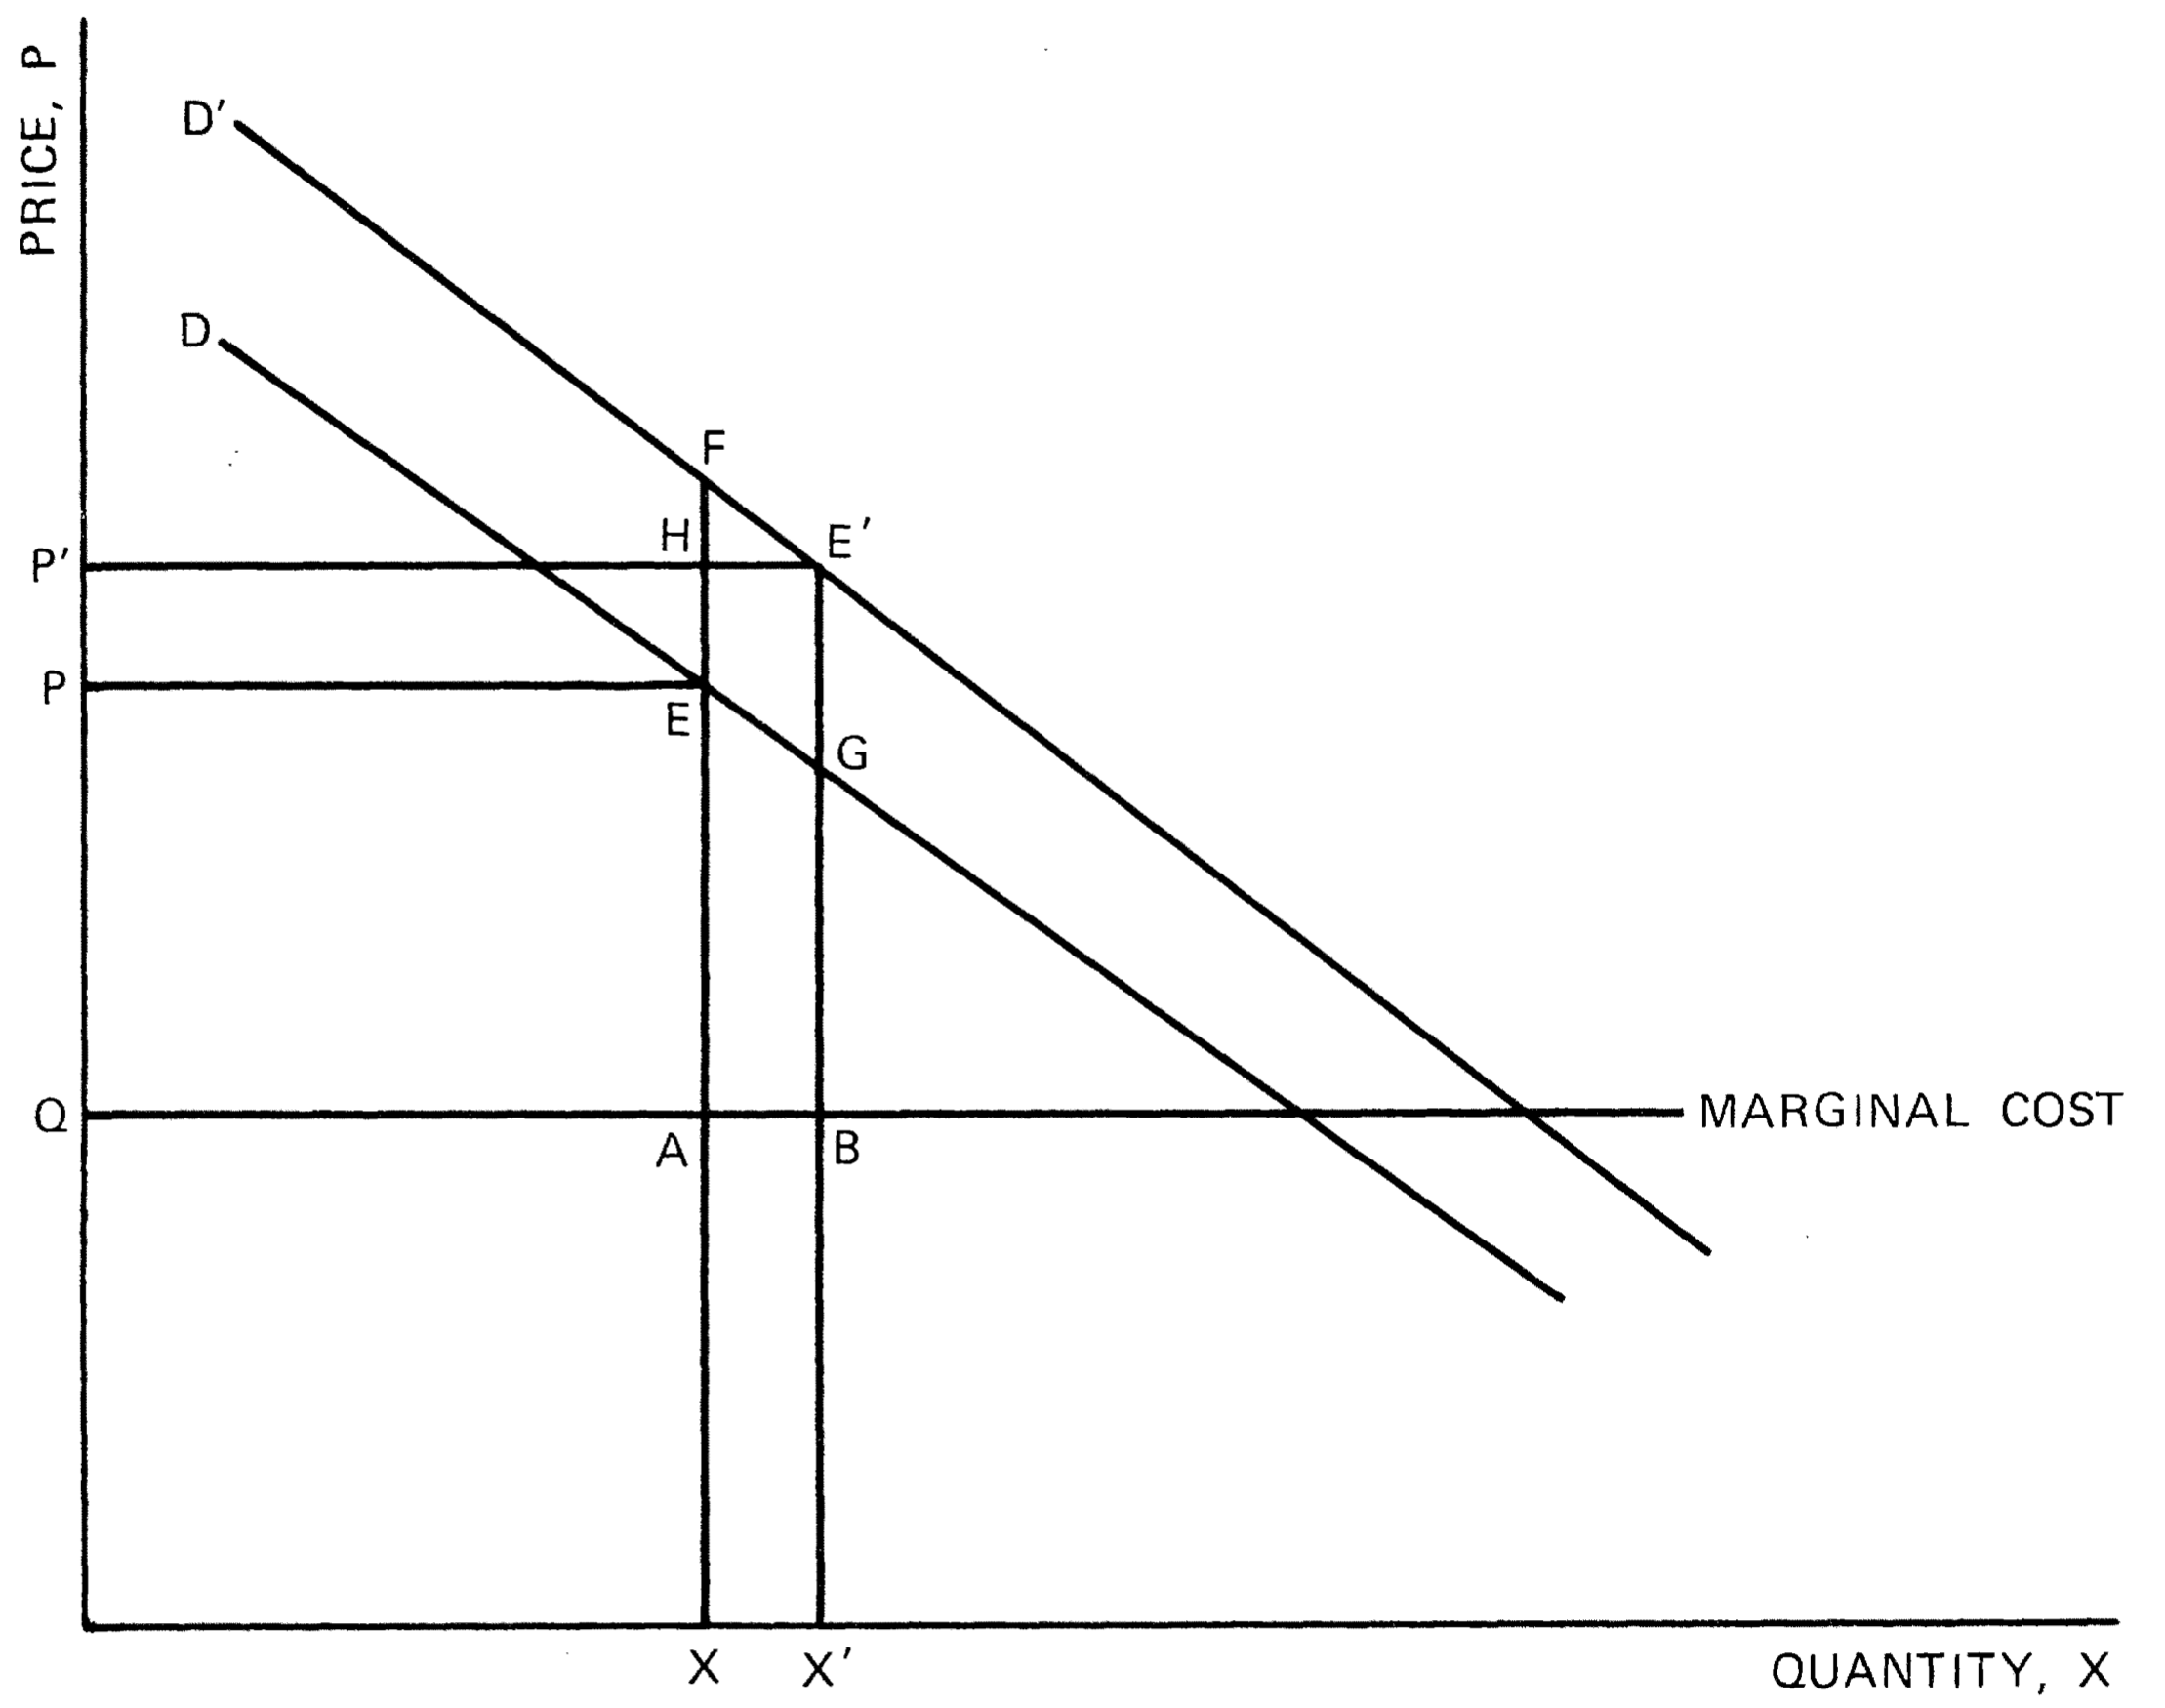
\includegraphics[width = .9\textwidth]{dixit.png}
\end{figure}
\end{frame}


\begin{frame}{Graphic Intuition}
Can consumer gain surplus from advertising?
\begin{figure}
    \centering
    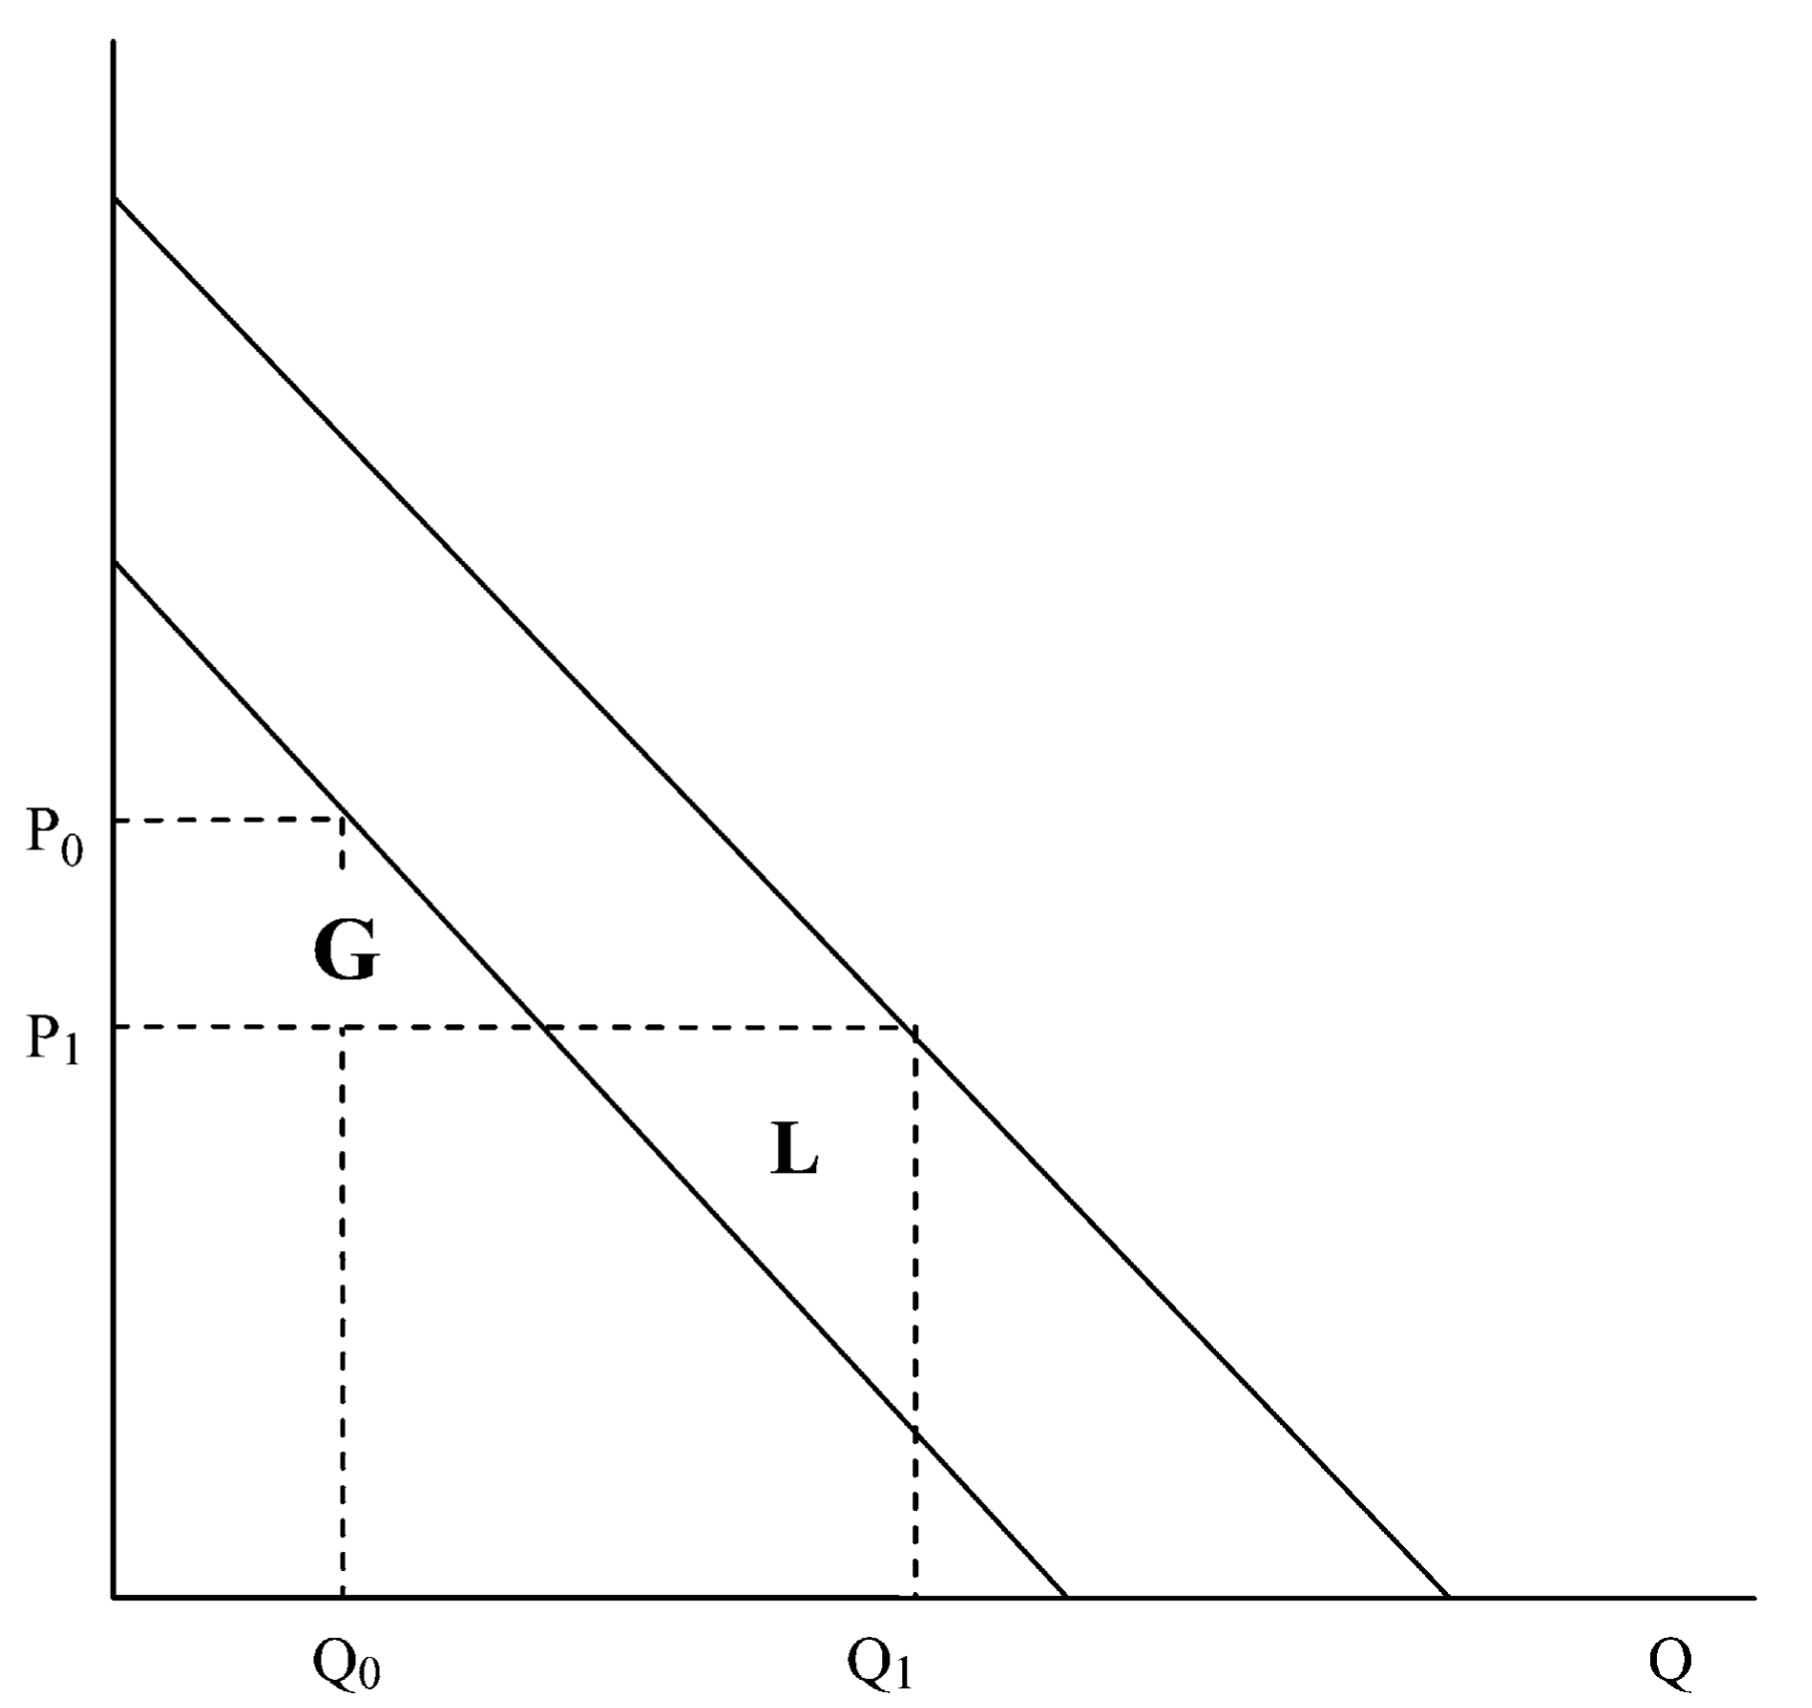
\includegraphics[width = .7\textwidth]{dixit2.png}
\end{figure}
\end{frame}

\begin{frame}{Dixit \& Norman}
    In a "formaly" way, after a change of advertising level, 
    \begin{equation}
        \Delta W = \Delta \pi - x \Delta p
    \end{equation}

    From this equation we can see that if firm maximized their prifit, i.e., $\Delta \pi = 0$, and if $\Delta p < 0$, we have $\Delta W > 0$
\end{frame}

\subsection{Empirical Findings and New Direction}
\begin{frame}{Empirical Findings}
Empirical studies on advertising is usually questioned by two obstacles: endogeneity concern and measurement problem.
\begin{enumerate}
    \item High advertising level may be associated with a lot of variables: sales, inelastic demand, high profitability, low cost, etc. Most of the time, those \textcolor{red}{variables are tangled}. Also the \textcolor{red}{simultaneous causality} is also worrisome.
    
    \item As for measurement, advertising intensity can be hard to measure. Current level or accumulated level? Current expense or intangible capital?
\end{enumerate}

Given all this difficulties, empirical studies still are very important since we can use them to verify different views.
\end{frame}

\begin{frame}{Empirical Findings}
Some aspects that people have studied:
\begin{itemize}
    \item Sales \\
    Is there a positive association between current advertising and current and future sales? Does it increase demand at industry level or redistribute within industry?
    \item Brand loyalty(market share stability)\\
    Estimate demand funtion to check elasticity in different industries; examine the adverting-market-share-stability relationship
    
    \item Advertising scale of economy\\
    Marginal effectness of generating revenue; expenditure per message
    \item Market concentration\\
    Advertising and market power

\end{itemize}
\end{frame}

\begin{frame}{Empirical Findings}
    \begin{itemize}
        \item Profit\\
        How to interpret profit-advertising relationship?
        \item Entry\\
        Some believe ads do deter entry, while some don't
        \item Price\\
        Some believe advertising increase retail price, while other think it might decrease it due to lowering searching cost.
        \item Quality \\
        Positive relationship between advertising and product quality is observed, but the relationship fails in some circumstances
    \end{itemize}
\end{frame}

\begin{frame}{New Directions--Two-sided Market}
Advertising and media markets: there are many platforms for whom commercial advertising is a major source of income. 

Two-sided market: two groups interact through an intermediary or platform. For example: TV market, credit card, and nowadays social media, video platform, livestream. 

We can generalize it in a three-party interaction: \textcolor{red}{the advertiser}, \textcolor{red}{the platform}, and \textcolor{red}{the users}.

On the one hand, the advertisers are benefited when there are many users of the platform. On the other hand, the users may get negative utility from the ads.
\end{frame}

\begin{frame}{New Directions--Two-sided Market}
Several commentators argue that, over the past several years, firms have increasingly opted for ads that target specific consumer groups.

It's reasonable since we can imagine that targeted advertising has higher rate of return. It works like price discrimination.

However, the way they match the ads to each consumer is based on personal informaiton, eg. news preference, shopping history, google map trace, social media post. it leads to direct concern of privacy.
\end{frame}

\begin{frame}{New Directions--Behavioral Econ}
As we've seen a lot of models based on advertising altering consumers' taset and preference, but how it works?

This strand of research use psychological and neuroscience findings to understand economic decisions and model new insights.
    
\end{frame}






\end{document}
